% =====================================================================
% ICBINB-BIO @ NeurIPS 2026  --  paper (official workshop style)
% ---------------------------------------------------------------------
% Upload main.tex, supplementary.tex, neurips_2026.sty, the bibliography in
% Literature_Sources/, and the figure PDFs referenced below. Set main.tex as
% the main document. The appendix is compiled into the submission PDF.
%
% SUBMISSION (double-blind): keep the [dblblindworkshop] option below.
% CAMERA-READY (after accept): switch to [dblblindworkshop, final].
% =====================================================================
\documentclass{article}

% Numbered citations [1] (standard NeurIPS look) -- must precede neurips_2026:
\PassOptionsToPackage{numbers,sort&compress}{natbib}

% Double-blind workshop submission (auto-anonymizes the author block below).
% Submission (anonymous):   \usepackage[dblblindworkshop]{neurips_2026}
\usepackage[dblblindworkshop, final]{neurips_2026}
% Preprint / arXiv (non-anon):                       \usepackage[preprint]{neurips_2026}

% Required: the workshop title shown in the footnote.
\workshoptitle{I Can't Believe It's Not Better (ICBINB): Failure Modes of AI in Biology}

\usepackage[utf8]{inputenc}
\usepackage[T1]{fontenc}
\usepackage{hyperref}
\hypersetup{hidelinks}
\usepackage{url}
\usepackage{booktabs}
\usepackage{amsmath,amssymb,amsfonts}
\usepackage{nicefrac}
\usepackage{microtype}
\usepackage{xcolor}
\usepackage{graphicx}
\usepackage{placeins}   % \FloatBarrier: keep main-text floats out of the appendix
% Camera-ready revision marking: wrap changed text in \rev{...} to show it in red.
% Set \revoff to typeset the final version in black.
% \color (a switch) rather than \textcolor (an argument), so a \rev{...} may
% span more than one paragraph without "Paragraph ended before \@textcolor".
\newcommand{\rev}[1]{\begingroup\color{red}#1\endgroup}
%\renewcommand{\rev}[1]{#1}  % <- uncomment for the final black version

% --- float placement: the two main figures are tall (full-width multi-panel
% --- plus a long caption), so the defaults push them onto deferred float pages.
\renewcommand{\topfraction}{0.95}
\renewcommand{\bottomfraction}{0.7}
\renewcommand{\textfraction}{0.05}
% a float page must be >=90% full, so a tall figure goes at the top of a text
% page instead of claiming a page of its own
\renewcommand{\floatpagefraction}{0.90}
\setcounter{topnumber}{2}
\setcounter{totalnumber}{4}

\title{Composition Without Grammar: Next-Token Models Miss Regulatory Structure in Bacterial DNA}

% Camera-ready author block.
\author{%
  Marc Augustine Sojerido Amil \\
  King's College London \\
  \texttt{marc.amil@kcl.ac.uk} \\
  \And
  Aleksej Zelezniak \\
  King's College London \\
  and Chalmers University of Technology \\
  \texttt{aleksej.zelezniak@kcl.ac.uk} \\
  \texttt{aleksej.zelezniak@chalmers.se} \\
}

\begin{document}
\maketitle

\begin{abstract}
Natural selection jointly shapes bacterial genes and their cis-regulatory
contexts. Context-aware regulatory-sequence design therefore requires more than
generating species-typical DNA: upstream regions must encode valid positional
grammar and, where relevant, be compatible with the target coding sequence.
Because genomic language models are trained on complete genomes, one might expect
them to capture these dependencies. We assess whether these models capture local,
position-dependent promoter grammar and statistical associations between coding
sequence (CDS) and its upstream region. In a comparative analysis of singleton
orthologues, upstream similarity increased with CDS relatedness, whereas matched
non-homologous controls showed little association. Motivated by this observation,
we evaluate three tasks in \emph{E.~coli} and \emph{B.~subtilis}: promoter-element
placement, CDS-conditioned upstream generation, and retrieval of the native
upstream among 99 decoys. Across five autoregressive models, promoter
placement was comparable to shuffled controls. After fine-tuning Evo with a
species token, generated sequences reflected the base composition of the requested
species and included a Shine--Dalgarno signal. However, replacing, shuffling, or
removing the CDS produced only small changes in the generated upstream. Lastly, in the
retrieval task, the best autoregressive model ranked the native upstream first in
$6.3\%$ of cases. By contrast, the contrastively trained C3P model reached
$82.7\%$ on \emph{E.~coli}, which was excluded from its training set. Under the
evaluated settings, next-token models therefore capture broad composition more
readily than motif identity, spacing, or gene-specific association, whereas a
contrastively trained model can exploit the pairwise signal.
\end{abstract}

% =====================================================================
\section{Introduction}
\label{sec:intro}
Regulatory regions and the genes they control are shaped by related evolutionary
pressures. Previous work has identified coordinated evolutionary patterns between
coding sequences and their upstream regulatory contexts, reflecting selection
associated with gene function, expression requirements, cellular cost and the
regulatory machinery of the
host~\citep{zrimec2020coevolution,zrimec2021regulatorycode}. Near the translation start site, this relationship is further
shaped by direct sequence-level constraints involving RNA structure, codon choice
and translation initiation~\citep{salis2009rbs,kudla2009coding,
cambray2018translation}. These associations are also apparent in a simple
comparison of orthologous genes (Fig.~\ref{fig:setup}A;
Appendix~\ref{app:fig1a}). Across $22{,}393$ pairs of
orthologues representing monocistronic genes from $408$ gammaproteobacterial
genomes, nucleotide identity at third codon positions---a measure of CDS
relatedness that is less constrained by amino-acid conservation---was positively
correlated with the $k$-mer similarity of the corresponding $200$\,bp upstream
regions (Spearman's $\rho=0.437$, $p<10^{-300}$). Length-matched pairs of
non-homologous monocistronic genes from the same genomes showed little correlation
($\rho=0.027$, $p=4.7\times10^{-5}$), suggesting that broad differences in GC
content, codon usage and promoter composition alone do not explain this pattern.
More closely related coding sequences therefore tend to be accompanied by more
similar upstream regions, raising the question of whether genomic language models
learn this association.

Genomic language models are trained on complete genomes containing coding and
regulatory sequence and could, in principle, learn this association. They are
increasingly used to generate sequences ranging from regulatory elements to
complete CRISPR--Cas systems and genome-scale DNA
~\citep{nguyen2024evo,brixi2025evo2,promogen2}. We ask two questions
in this work.  Local promoter grammar asks
whether a model learns motif identity and positional relationships such as
distal--proximal box spacing. Gene conditioning asks whether it understands the
longer-range association between an upstream region and a particular CDS, rather
than producing a generic species-typical sequence.

These capabilities may be challenging for next-token prediction as a
bacterial upstream contains a few short, identifiable elements---promoter boxes, the
Shine--Dalgarno sequence and binding sites---within a larger spacer
background~\citep{ross1993up,spacer2021,salis2009rbs,regulondb2024}, and cross-entropy
weights every position equally (\S\ref{sec:why}). Related evidence comes from
perturbing natural sequences and evaluating their
likelihoods~\citep{invariance2026}. Here we instead ask the models to write
upstream sequence, also testing long-range dependence between the CDS and its
upstream region.

\paragraph{This paper.}
Motivated by Fig.~\ref{fig:setup}A, we ask whether
autoregressive DNA models write upstream sequences with the annotated local elements
and whether their predictions depend on the particular CDS. Three tasks
(Fig.~\ref{fig:setup}B--D) test this: promoter-grammar completion
(\S\ref{sec:upstream}), CDS-conditioned generation from a fine-tuned
Evo~\citep{nguyen2024evo} (\S\ref{sec:cds}), and recognition of the true upstream
among $99$ same-genome decoys (\S\ref{sec:retrieval}). After evaluation, we find limited
evidence for either capability: the models reproduce
broad composition but show little evidence of consistent promoter-element
placement or sensitivity to the supplied CDS. A model trained by contrastive loss shows that the pairwise signal 
between CDS and upstream  can be recovered with a different objective.

\begin{figure}[!htb]
  \centering
  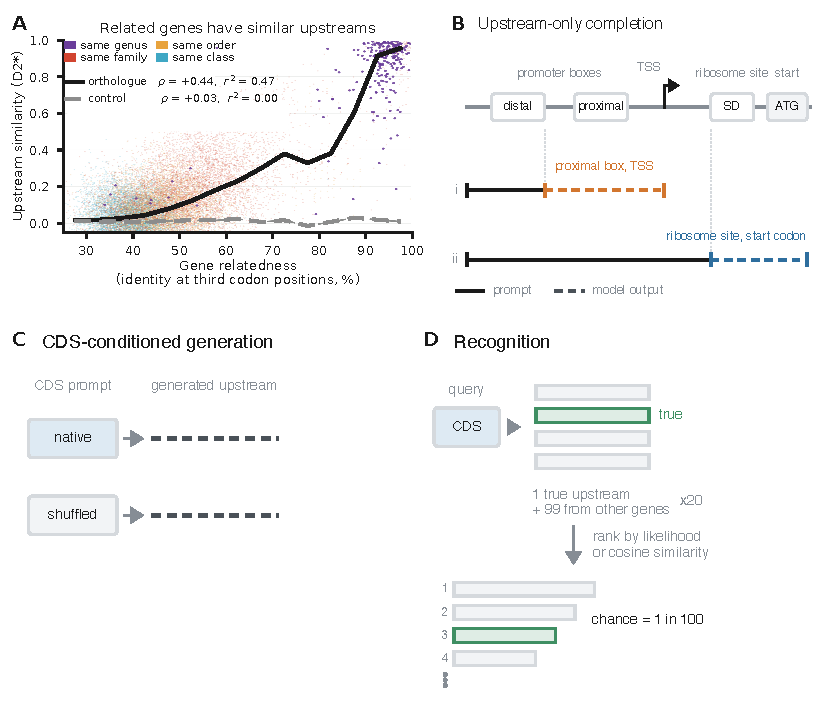
\includegraphics[width=\linewidth]{figures/Fig1_setup.pdf}
  \caption{\textbf{Gene--upstream association and the three evaluation tasks.}
  \textbf{(A)}~Each point is one \emph{E.~coli} K-12 singleton gene paired with a
  singleton orthologue in another Gammaproteobacterial genome ($22{,}393$ pairs,
  $408$ genomes; \rev{both genes have an operon size of one and at least
  $200$\,bp to the nearest upstream feature, so every window is intergenic}): identity at third codon positions against alignment-free
  similarity ($D_2^*$, $4$-mers against an order-2 Markov background) of the two
  $200$\,bp upstream regions. Colour is the target genome's taxonomic rank relative
  to \emph{E.~coli}; curves are running medians for orthologues (black) and for a
  length-matched non-homologous singleton from the same genome (grey dashed).
  \textbf{(B)}~\emph{Upstream-only completion} (\S\ref{sec:upstream}). A map of the
  upstream region with two prompt cut points: in~(i) the prompt ends at the distal
  box and the model writes the proximal box and the transcription start site (TSS,
  orange); in~(ii) it ends before the Shine--Dalgarno and the model writes the SD
  and the start codon (blue). Solid lines mark the prompt, dashed lines what the
  model generates.
  \textbf{(C)}~\emph{CDS-conditioned generation} (\S\ref{sec:cds}). The model
  generates the upstream from the native coding sequence and repeated with the CDS composition
  shuffled.
  \textbf{(D)}~\emph{Recognition} (\S\ref{sec:retrieval}). For a query CDS, the true
  upstream (green) is ranked against $99$ upstreams of other genes (grey), by
  likelihood or by embedding cosine similarity, over $20$ decoy sets per gene;
  chance is 1-in-100.}
  \label{fig:setup}
\end{figure}

% =====================================================================
\section{Problem, hypotheses and evaluation design}
\label{sec:setup}

\paragraph{Biological task and data.}
The target is not exact reconstruction of one native upstream sequence, as generating the specific 200\,bp sequence base for base is a hard problem. Instead, the evaluation measures two dependencies:
local element identity and spacing, and a distributional response to the gene
being regulated. The
\emph{upstream-only} track contains $671$ \emph{E.~coli} K-12 MG1655 genes with
up to 200\,bp upstream, RegulonDB annotations~\citep{regulondb2024}, and assignments
to one of five sufficiently represented sigma factors
(Appendix~\ref{app:benchmark-composition}). Since \emph{E.~coli} K-12 MG1655 occurs in
several pretraining corpora, each prompt has a \emph{leaked} version containing
the natural sequence and a \emph{clean} version that retains all annotated
elements, such as the proximal and distal box, at their native positions while shuffling the other bases. The
\emph{CDS-prompted} track contains every qualifying singleton gene with a complete
200\,bp upstream in \emph{E.~coli} MG1655 ($1{,}885$) and \emph{B.~subtilis} 168
($1{,}272$; Appendix~\ref{app:cds-composition}). The retrieval track evaluates
$500$ \emph{E.~coli} singletons, whose upstream reaches a full $200$\,bp before the neighbouring gene---each against
$99$ same-genome decoys over $20$ resamples.

\paragraph{Models and evaluation approach.}
The upstream-only track uses five published autoregressive DNA checkpoints with
their weights unchanged: Evo\,1 at both released context lengths, 8k and 131k
(\texttt{evo-1-8k-base}, \texttt{evo-1-131k-base})~\citep{nguyen2024evo}, Evo\,2
(\texttt{evo2\_1b\_base})~\citep{brixi2025evo2}, HyenaDNA
(\texttt{hyenadna-medium-450k-seqlen})~\citep{nguyen2023hyenadna} and PromoGen2
(\texttt{promogen2-base})~\citep{promogen2}. All but HyenaDNA, which was trained on
human hg38, saw bacterial genomes in pretraining. The CDS-prompted track evaluates
fine-tuned \texttt{evo-1-8k-base}. Recognition additionally uses frozen C3P (100M),
a contrastive promoter--protein model pretrained on 88 million bacterial pairs with
\emph{E.~coli} held out~\citep{dufault2026c3p}; it is used for retrieval and not as a
generator. Every generative prompt is decoded 20 times at $T=1.0$.

\paragraph{Hypotheses and failure criteria.}
Under \textbf{H1}, a model has learned local grammar if it places a
same-sigma-factor proximal box within $\pm2$\,bp of the annotation more often than
composition-preserving controls, and recovers its bases at the annotated position
(\emph{placement} and \emph{motif identity}, Appendix~\ref{app:metrics}). The
$\pm2$\,bp window is a loose reading of a tight biological constraint: in real
$\sigma^{70}$ promoters the distal--proximal spacer is sharply peaked, sitting in
the canonical $15$--$19$\,bp window $60.5\%$ of the time
(Fig.~\ref{fig:spacerhist}).
Under \textbf{H2}, a conditional generator uses the gene if the upstream it writes
changes when the prompted CDS changes. We generate under two prompt conditions,
the native CDS and a shuffled version of that same CDS, and compare the two sets
of upstreams by KL divergence (Appendix~\ref{app:metrics}). Retrieval checks the
same dependence without generating anything: top-1 accuracy should exceed the
1-in-100 chance rate when all decoys come from the same genome.

\paragraph{CDS-conditioned fine-tuning.}
We fine-tuned Evo on bacterial genes with the coding sequence first and the
upstream after it---\texttt{+\#CDS+\$upstream} for \emph{E.~coli} and
\texttt{@\#CDS@\$upstream} for \emph{B.~subtilis}. The objective is plain
next-token cross-entropy with no masking.\texttt{+} and \texttt{@} correspond to the species token
to generate species-specific sequences. The CDS$\rightarrow$upstream order reverses natural left-to-right genome modelling but
is required for causal conditioning: an autoregressive model predicts only later
tokens, so the CDS must precede every upstream token. This conditional design
follows control-token generators~\citep{madani2023progen,
munsamy2024zymctrl,lal2024reglm,promogen2}. It also matches the practical case: a
user typically has a protein they want expressed and needs regulatory sequence to
drive it, so the CDS is the given and the upstream is what the model must
supply.

\paragraph{Retrieval scoring.}
Autoregressive models are evaluated using candidate-centred conditional log
likelihood and centred cosine similarity between CDS and upstream embeddings.
C3P instead uses protein--upstream cosine similarity
(Appendix~\ref{app:metrics}). Rank $1$ places the native upstream above all $99$
decoys.


% =====================================================================
\section{Observed outcome I: models miss promoter-element placement}
\label{sec:upstream}

The first task tests whether the models can generate a real upstream sequence given the prompt of the end of the
distal box. It must write the proximal box with the correct spacing, which is
tightly constrained. We locate the box by taking the highest-scoring
position-weight-matrix (PWM) window of the proximal box in the generation and count it correct if it falls
within $\pm2$\,bp of the annotated position; the same high scoring PWM is also used to assess base comparisons
to the true bases of the proximal box scored in Fig.~\ref{fig:upstream}C (Appendix~\ref{app:metrics}).

\begin{figure}[tbp]
  \centering
  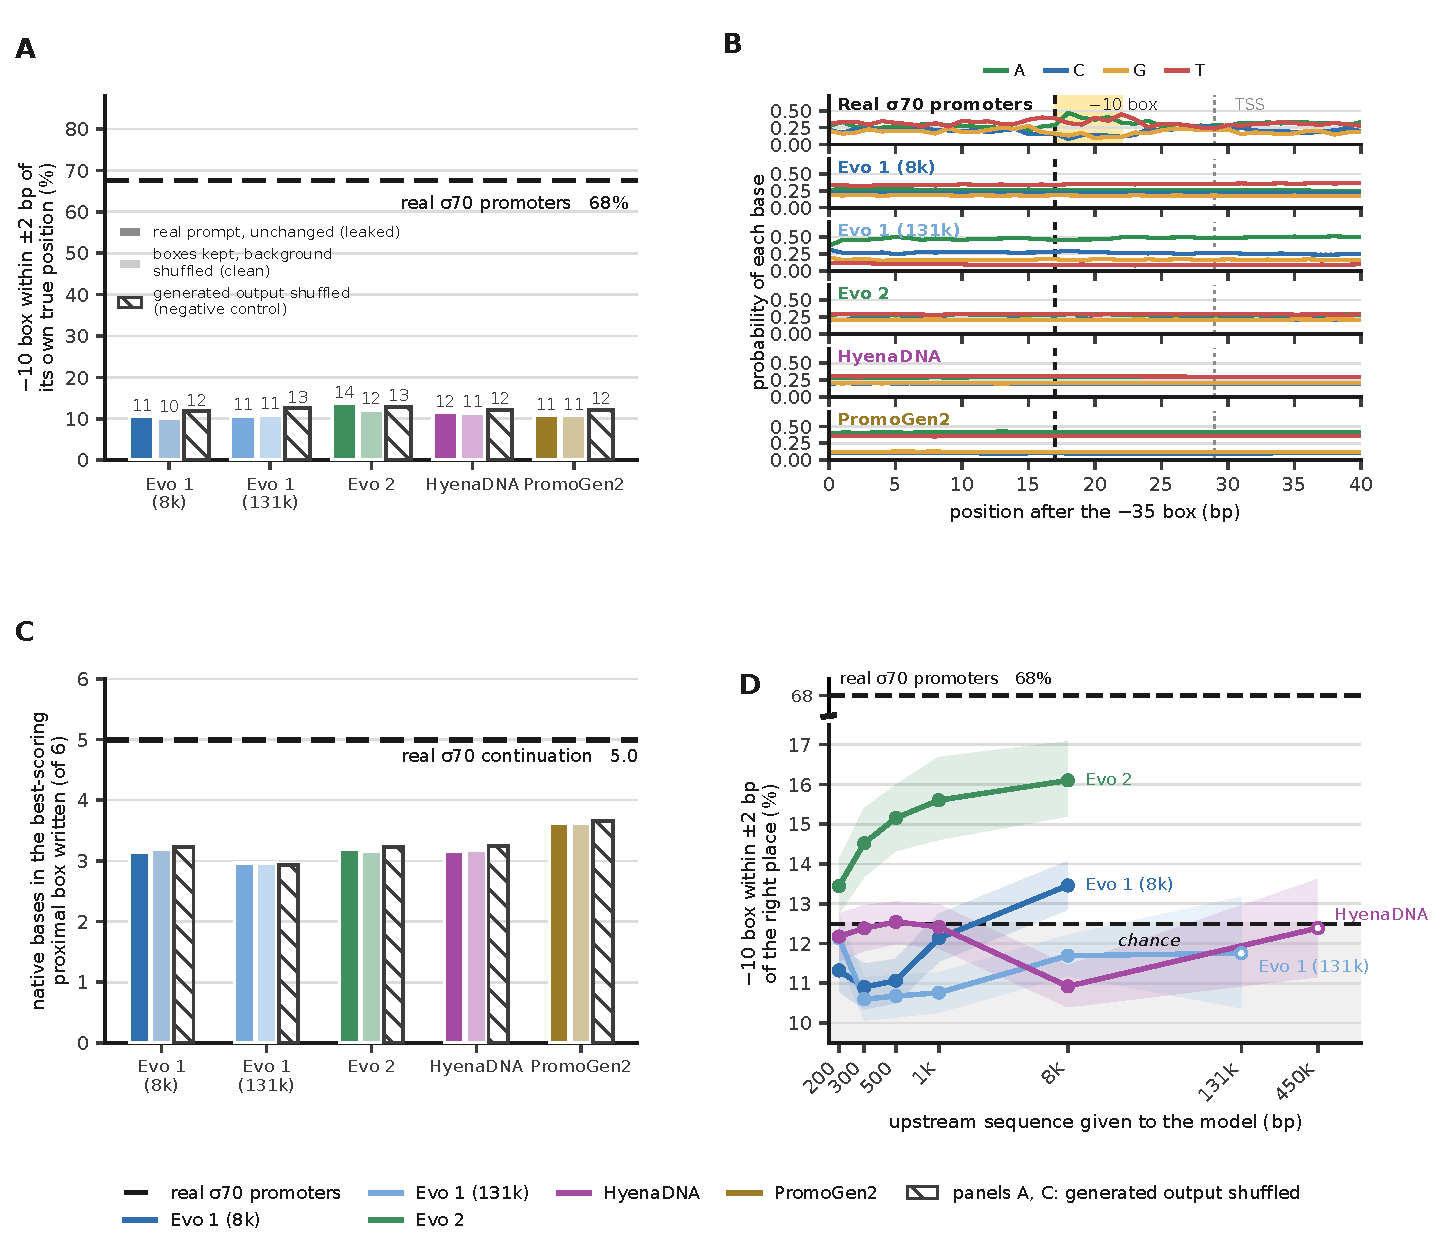
\includegraphics[width=\linewidth]{figures/fig_upstream_only_v2.pdf}
  \caption{\textbf{Promoter-element placement after upstream completion.}
  Five checkpoints continued \emph{E.~coli} $\sigma^{70}$ upstreams from the end
  of the distal box (20 generations per promoter, $T=1.0$).
  \textbf{(A)} Does the proximal box land in the right place? Fraction with a
  proximal-box PWM match within $\pm2$\,bp of the annotation, for natural, clean
  and shuffled-output conditions.
  \textbf{(B)} Real sequence has a signal at the proximal box that model cannot capture.
  Mean base probabilities over the $41$\,bp following the distal box, which spans
  the proximal box and the TSS.
  \textbf{(C)} Do the highest-PWM box bases match the true proximal-box bases? Mean
  bases of the highest-scoring proximal-box PWM window in each generation that
  match the gene's annotated box.
  \textbf{(D)} More context does not fix it. Placement accuracy as prompt context
  increases. Shading gives $95\%$
  confidence intervals.}
  \label{fig:upstream}
\end{figure}


\paragraph{No tested checkpoint writes or places the proximal box correctly.}
All models place the proximal box near the shuffled baseline
(Fig.~\ref{fig:upstream}A; per-sigma-factor values in Table~\ref{tab:upstream}),
whereas the identical scan
recovers the annotated position in $68\%$ of real promoters. For four of five
checkpoints, scrambling the generated output gives an equal or higher score, so
base order adds little information about box position. The space between distal and proximal box
distribution for real promoters is sharply peaked at $17$\,bp, whereas the
distribution from every model is nearly flat across the scanned window
(Fig.~\ref{fig:spacerhist}). Accordingly, a $17$\,bp spacer occurs in $21.0\%$ of
real promoters but only $2.0$--$3.0\%$ of model generations, close to the $2.5\%$
expected from uniform placement. The models are therefore not simply missing the
annotated position by a few bases; they fail to capture the narrow spacer-length
constraint of real $\sigma^{70}$ promoters. Access to a potentially
memorised genomic background does not rescue performance: Evo\,1 and Evo\,2 saw
\emph{E.~coli} during pretraining, yet shuffling non-regulatory prompt bases while
preserving annotated elements changes placement by at most $1.6$ percentage
points and by $0.3$ points for Evo\,1 (8k). The bases are also incorrect. We take the highest-scoring
proximal-box PWM window anywhere in the generated $45$\,bp and compare its six
bases with that gene's annotated box. The same scan on the real continuation
scores $4.99/6$. Every checkpoint scores
$2.96$--$3.62/6$, inside the $2.94$--$3.65$ range of its own shuffled output
(Fig.~\ref{fig:upstream}C). So the best box a model writes is no closer to the
real one than a shuffle of its own output. The Shine--Dalgarno behaves the same
way: every model scores $2.6$--$3.0/6$ against $5.01/6$ for real sequence
(Fig.~\ref{fig:sd-placement}).


\paragraph{The models fit composition, not position.} Over the $41$\,bp following
the distal box, the four base probabilities remain flat: entropy changes at most
$0.03$ bits for four of the five models (Fig.~\ref{fig:upstream}B). Real
promoters do move, falling to $1.72$ bits inside the proximal box where A and T
reach $0.47$ and $0.45$. What the models get right is the average level: their mean
$P(\mathrm{A})+P(\mathrm{T})$ is $0.57$--$0.61$ against $0.62$ in real upstreams,
PromoGen2 aside at $0.78$. This reflects the training dataset of the models being
AT-rich in the non-coding DNA (Appendix~\ref{app:traincomp}).

The flatness is specific to regulatory sequence. Prompted at the midpoint of a
coding sequence instead, the same models write a profile that fluctuates from
position to position and follows a real CDS profile: Evo\,2 and Evo\,1 reach $0.21$ and
$0.88$ of a composition-only reference, against $1.05$ and $1.16$ on the upstream,
where $1$ means composition and nothing more (Appendix~\ref{app:cdscompletion}).
Coding sequence constrains most positions through reading frame, codon periodicity
and codon usage.

\paragraph{More context does not help.} The $200$\,bp window is not the limit:
extending the prompt to $300$, $500$ and $1000$\,bp, and on to each checkpoint's
trained limit --- up to $131$\,kb for \texttt{evo-1-131k-base} and $450$\,kb for
HyenaDNA --- leaves three of four models at chance and lifts Evo\,2 only to
$1.29\times$ chance (Fig.~\ref{fig:upstream}D). Beyond $200$\,bp there is little
regulatory sequence as the median \emph{E.~coli} gene has
only $203$\,bp of intergenic sequence in front of it, so a $1000$\,bp prompt runs
back into the neighbouring gene for $98.7\%$ of genes; the extra context is mostly
more coding sequence, not more regulation.



% =====================================================================
\FloatBarrier   % Table 1 and Fig. 2 must both appear before this section
\section{Observed outcome II: fine-tuning does not make next-token models CDS-sensitive}
\label{sec:cds}

\begin{figure}[!tbp]
  \centering
  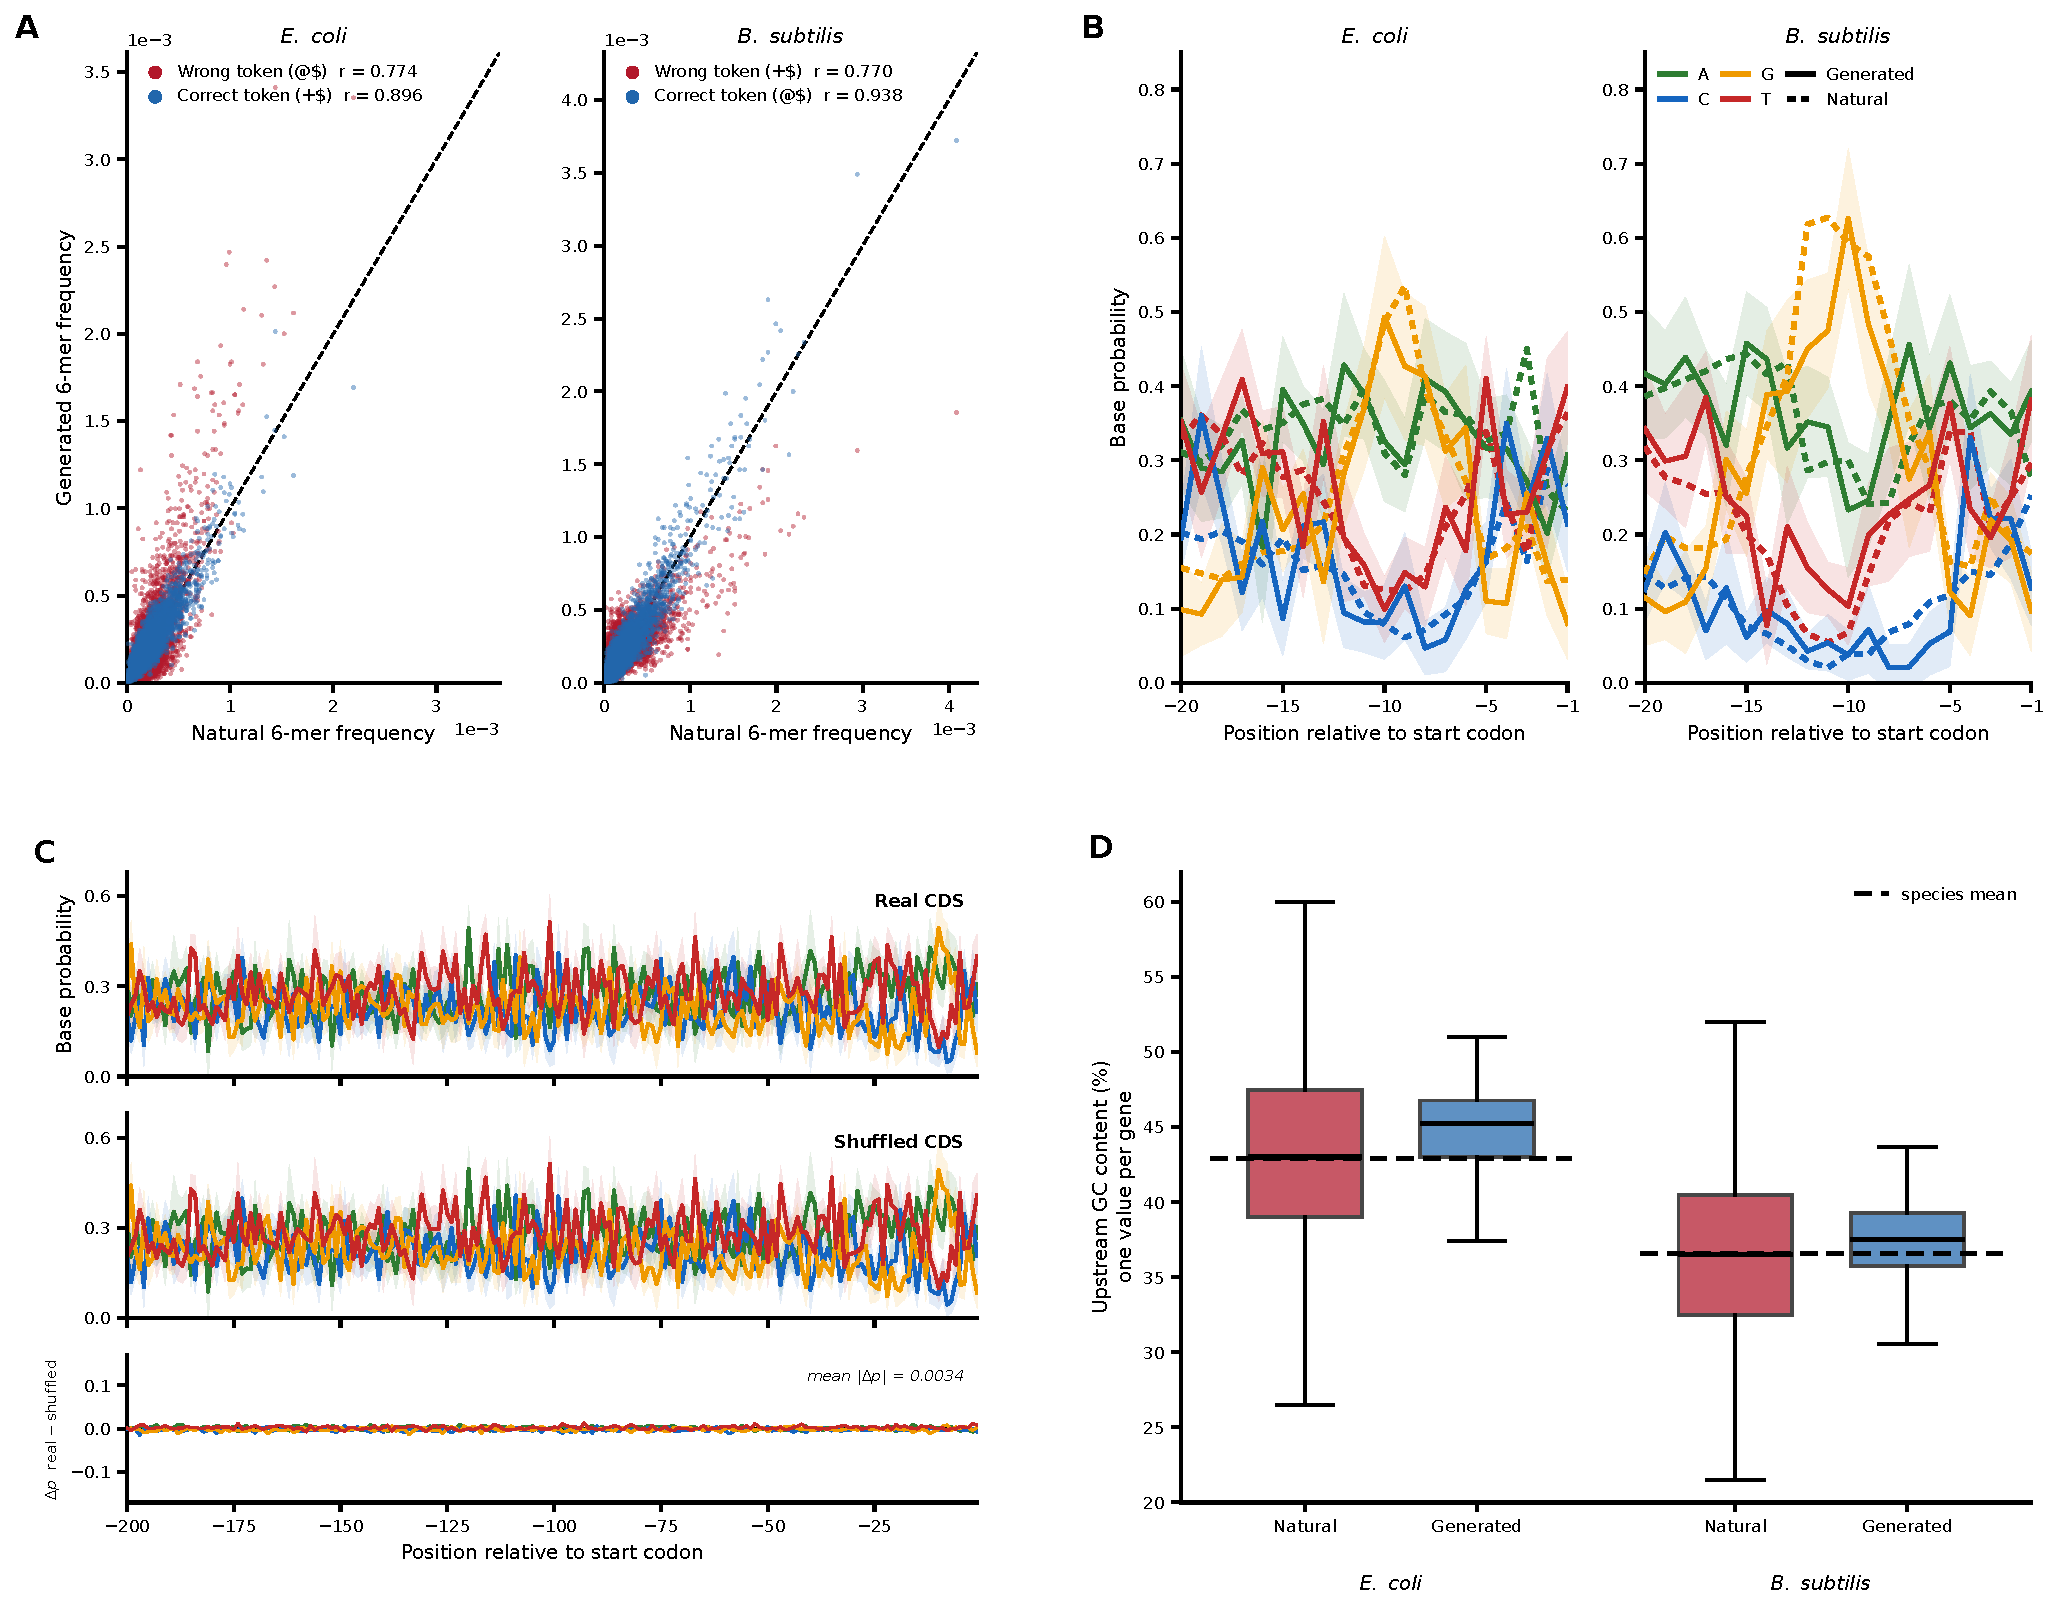
\includegraphics[width=\linewidth]{figures/cds_prompted_main.pdf}
  \caption{\textbf{Generated upstream properties and sensitivity to CDS perturbations.}
  All outputs use the fine-tuned checkpoint and $T=1.0$. Panels A and B use only
  a species token and the upstream marker (no CDS); panels C and D use CDS
  prompts. \textbf{(A)} Natural versus generated 6-mer frequencies under matched
  and mismatched species tokens ($673$ \emph{E.~coli} and $441$
  \emph{B.~subtilis} upstreams; 20 outputs each); Pearson $r$ is reported.
  \textbf{(B)} Positionwise natural (dashed) and generated (solid) base profiles
  near the Shine--Dalgarno region; shading is $\pm1$ standard deviation.
  \textbf{(C)} Base profiles under the native and shuffled CDS prompts, and their
  difference. \textbf{(D)} Per-gene GC content of natural upstreams and outputs
  generated from the native CDS prompt.}
  \label{fig:cds}
\end{figure}

Since the base autoregressive models performed poorly on promoter placement,
we fine-tuned Evo to test whether conditional training can recover both
species-level sequence and the gene--upstream association. During fine-tuning,
the model receives a species token followed by the coding sequence, then the
corresponding 200\,bp upstream region. Each example follows the format
\texttt{<sp>\#CDS<sp>\$upstream}, where \texttt{<sp>} identifies the species,
\texttt{\#} marks the CDS, and \texttt{\$} marks the start of the upstream
sequence. The experiment asks whether its distribution changes under controlled
CDS perturbations. For each gene, we generate 20 sequences at $T=1.0$ under the
seven conditions in Table~\ref{tab:conditions}, which differ only in the CDS. To separate the learned species prior
from CDS dependence, Fig.~\ref{fig:cds}A--B first omits the CDS entirely and
Fig.~\ref{fig:cds}C--D then analyzes CDS-prompted outputs.

\paragraph{The generator captures broad sequence patterns.}
Figure~\ref{fig:cds}A compares the frequency of each of the $4096$ possible
6-mers in generated and natural upstreams. Prompted with its own species token,
the model reproduces natural 6-mer frequencies closely ($r=0.896$ for
\emph{E.~coli}, $r=0.938$ for \emph{B.~subtilis}) compared with the other species' token
the correlation falls to $0.774$ and $0.770$, so the token carries species-level
information. This measure is position-blind, as a high 6-mer correlation is
achievable from composition alone and does not by itself indicate regulatory
grammar. 

The model captures the Shine-Dalgarno (SD) sequence. Figure~\ref{fig:cds}B shows base
probabilities over the final $20$\,bp before the start codon for natural (dashed)
and generated (solid) upstreams. The generated profiles track the natural ones in
both species, including the G peak near position $-10$, and capture the species-specific form: in real sequences the
peak reaches $0.63$ in \emph{B.~subtilis} against $0.54$ in \emph{E.~coli}, and
the generated profiles give $0.63$ against $0.49$. However, this feature is the easiest to capture, since the SD sequence sits at nearly the same offset in every gene
(Fig.~\ref{fig:benchmark-composition}B).

\paragraph{Changing the conditioning CDS has almost no effect on generation.}
In Figure~\ref{fig:cds}C we prompt the model with the real CDS and with a
shuffled version of that same CDS, which keeps its base composition but destroys
the gene it encodes. If the model were reading the gene, the two prompts should
lead it to write different upstreams. The first two tracks give the probability of
each base across the generated 200\,bp and are almost indistinguishable. The
third track subtracts one from the other and stays flat at zero, mean
$|\Delta p|=0.003$. Therefore, the CDS is present in the prompt but effectively absent
from the output. Table~\ref{tab:kl} puts the comparison in bits of
KL divergence, where zero means the CDS made no difference to what the model wrote.
Even deleting the CDS from the prompt entirely costs only $2.8$ bits over 200
positions, or $0.014$ bits per position. \rev{This is small rather than zero: a base
distribution can carry up to $2$ bits, so the most violent perturbation available
moves under $1\%$ of what could move. The response is also in the wrong place.
Fig.~\ref{fig:klpos} resolves it by position: it peaks in the first $50$ bases,
which the model writes immediately after reading the CDS, and decays with
distance, while the Shine--Dalgarno and start-codon region carries less than its
share of the window. The model therefore writes much the same upstream whatever
gene it is given, and what little it does condition on the CDS is spent away from
the positions that carry regulatory function.}

\paragraph{Generated upstreams have little gene-specific variation.}
Figure~\ref{fig:cds}D compares the GC content of natural and generated upstreams,
with one value for each gene. Natural upstreams vary substantially between
genes, with standard deviations of $6.6\%$ in \emph{E.~coli} and $5.4\%$ in
\emph{B.~subtilis}. Generated upstreams show less variation, with between-gene standard
deviations of only $2.3\%$ and $2.4\%$. Their GC values concentrate in the
high-density region of the corresponding natural distribution but span a
narrower range. The model therefore reproduces typical species-level composition
while under-representing the natural diversity among genes.

% =====================================================================
\FloatBarrier   % Fig. 3 must appear before this section
\section{Contrastive loss recovers pairwise signal}
\label{sec:retrieval}

Figure~\ref{fig:setup}A shows a relationship
between a gene and the upstream region. C3P model is introduced to assess if this pairwise 
signal can be captured by a model. C3P provides
such a reference: its 100M-parameter promoter encoder was contrastively aligned
to a frozen protein encoder on 88 million bacterial pairs, increasing similarity
for native promoter--protein pairs relative to mismatches. This pairwise loss
directly targets CDS--upstream association. C3P acts as a retrieval model, not a generator;
we use it only to test whether sequence contains a learnable pairing signal. We test on \emph{E.~coli}, a species that 
was excluded from the training set of C3P ~\citep{dufault2026c3p}. 

For each of the $500$ singleton \emph{E.~coli} genes in the retrieval set, we rank
the true upstream against $99$ same-genome decoys over $20$ resamples, scoring each
autoregressive model in two ways: candidate-centred likelihood and embedding
cosine similarity (Appendix~\ref{app:metrics}). Likelihood performs better;
Evo\,2 reaches $6.0\%$ top-1 by likelihood but $1.0\%$ by embedding.

C3P ranks the correct upstream first for $82.7\%$ of genes (median rank $1$),
providing a positive reference that the pairing is recoverable under a different
objective. Autoregressive top-1 accuracy
remains low: Evo\,1 $6.3\%$, Evo\,2 $6.0\%$, fine-tuned Evo $2.8\%$ and HyenaDNA
$1.0\%$ (median ranks $25$, $31$, $36$ and $47$, respectively). \rev{All of these
use the candidate-centred scorer, which subtracts each candidate's own
unconditional likelihood so that a generically likely upstream cannot win on
composition alone. Removing that correction raises Evo\,2 from $6.0\%$ to
$7.5\%$---the highest autoregressive value we measured, and still an order of
magnitude below C3P (Appendix~\ref{app:metrics}).}

\begin{figure}[tbp]
  \centering
  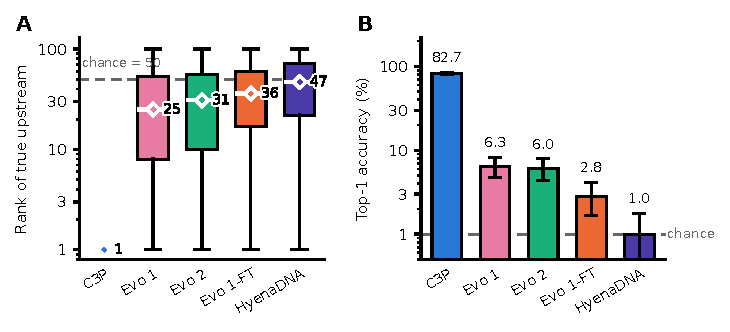
\includegraphics[width=\linewidth]{figures/fig_retrieval.pdf}
  \caption{\textbf{Retrieval of matched CDS--upstream pairs.} For $500$
  \emph{E.~coli} genes, the true 200-bp upstream was ranked among 99 same-genome
  decoys over 20 resamples. C3P uses protein--upstream cosine similarity;
  autoregressive models use candidate-centred conditional log likelihood.
  \textbf{(A)} Rank
  distributions (diamond, median; box, IQR; whiskers, $1.5\times$IQR).
  \textbf{(B)} Top-1 accuracy with 95\% bootstrap intervals; the dashed line marks
  chance. Two CDSs longer than $4.3$\,kb were excluded as queries but retained as
  decoys.}
  \label{fig:retrieval}
\end{figure}

% =====================================================================
\section{Failure analysis, boundary conditions and lessons}
\label{sec:why}

Next-token cross-entropy is a good objective function \rev{when selection
constrains most of the sequence.} In a protein, nearly every residue is under selection---for
fold, stability or activity---so a model that predicts the next residue better is
also a model that has learned more about the protein, and the two objectives
cannot be separated. This is why the same loss yields protein models that recover
structure and fitness~\citep{esm1v_meier2021,progen2_nijkamp2023,madani2023progen}. However, a bacterial upstream contains a small number of identifiable
elements including distal and proximal promoter boxes, the SD sequence, and transcription-factor
binding sites---embedded within spacer sequence that makes up most of the region. These
elements are also diverse and evolutionarily flexible. \rev{This motivates a hypothesis, which our measurements are
consistent with but do not establish: because next-token cross-entropy is summed
over every position, most of the training signal comes from the largely
unconstrained background rather than from the short identifiable elements, so
lower-order properties such as GC content and $k$-mer composition offer an easier
way to reduce the loss than motif identity and spacing. We state this as a
hypothesis because none of our experiments manipulate the objective. Testing it
requires an objective-level ablation---for instance re-weighting the loss at
annotated element positions, holding data and architecture fixed---which we do
not perform here.}

What the models write are flat profiles of AT-rich elements for the regulatory sequence. Across the $41$\,bp that span the
proximal box the probability of each base changes slightly with position
(Fig.~\ref{fig:upstream}B): real promoters dip to $1.72$ bits of entropy inside
the box, while no model moves by more than $0.03$ bits. The level they
settle at is close to correct, $58$--$60\%$ AT against $61.5\%$ in real upstreams,
and this is already the composition of their training data. The non-coding
sequence of all three corpora is AT-rich ($50.8\%$, $54.7\%$ and $59.2\%$ AT for
Evo\,1, Evo\,2 and HyenaDNA; Fig.~\ref{fig:traincomp}), and HyenaDNA arrives at
the same output composition having seen only human sequence. The same measurement on coding sequence gives the
opposite result: prompted at the midpoint of a CDS, these models write a profile
that varies from position to position and follows a similar profile to natural CDS sequences
(Appendix~\ref{app:cdscompletion}). Most bases in a CDS are constrained by the
genetic code, whereas identifiable regulatory elements occupy only about 20 of
the 200 upstream bases. \rev{This contrast is what the hypothesis above would predict: patterns present at
most positions are learned more readily than sparse, short regulatory
grammar}~\citep{simplicitybias2024,increasingcomplexity2024}. \rev{It is also
consistent with two accounts we cannot separate from it here. First, free-running
decoding compounds error---once a spacer drifts from its canonical length nothing
restores it---which is a property of sampling rather than of the training
objective. Second, uniform position weighting is shared by masked genomic
language models, so these results may reflect a limit of likelihood pretraining
on this class of sequence rather than of next-token prediction specifically.} 

Among the \rev{evaluated} models, Evo\,2 is the
only best-performing model that generates real CDS profiles in
the coding-sequence control (Appendix~\ref{app:cdscompletion}). Evo\,2's training procedure may contribute to this difference. Its initial
short-context training upweights genic windows, after which midtraining uses
longer sequences and a greater proportion of whole genomes~\citep{brixi2025evo2}.
This emphasis on gene-rich sequence may help explain Evo\,2's stronger performance
in the CDS control. More generally, the result supports that a model learns most
reliably the sequence properties emphasized during training.

\rev{\paragraph{Where this account is incomplete.}
PromoGen2 is the natural exception. It was trained on curated promoter sequence,
where regulatory elements are not sparse, so the hypothesis above predicts that
it should succeed. It does not: it places the $\sigma^{70}$ proximal box in
$10.8\%$ of generations and recovers the Shine--Dalgarno in $12.4\%$, both below
its own scrambled control ($12.3\%$ and $14.5\%$; Table~\ref{tab:upstream}).
Either the sparsity account is incomplete, or this checkpoint is being run
outside its intended use as a conditional design model. Two further limits bound
what we can claim. Evo\,2 appears at a single scale ($1$B), so the monotonic rise
of its placement accuracy with context (Fig.~\ref{fig:upstream}D) cannot
distinguish an objective that does not learn positional grammar from checkpoints
that did not. And fine-tuning \emph{lowered} retrieval, from $6.3\%$ for base
Evo\,1 to $2.8\%$; Fig.~\ref{fig:cds}D indicates why, as the between-gene
standard deviation of GC content falls from $6.6\%$ to $2.3\%$, making generated
upstreams more species-typical and less gene-specific.}

\paragraph{What these results do not show.}
Everything here is measured on sequence. We show that a gene and its upstream
carry matching statistical signal, and that some models can pick that signal up.
We do not show that a gene causes its promoter to look a particular way,
that a retrieved pair would express well, or that any generated upstream would
work in a cell. 

\paragraph{The obvious next model is a hybrid.}
The two objectives fail and succeed in complementary places. Cross-entropy writes
sequence but is dominated by composition; the contrastive loss cannot write
anything, yet it is the only objective here that ties a gene to its own upstream
($82.7\%$ against $6.3\%$ \rev{under the primary scoring rule and $7.5\%$ under
the most favourable variant}, Fig.~\ref{fig:retrieval}). The direct test is to train one
model under both at once: the same next-token cross-entropy, unchanged, plus a
contrastive term that scores each gene against its own upstream and against the
upstreams of other genes in the same genome. Cross-entropy keeps the ability to
write sequence; the contrastive term adds the gene--upstream pairing that
cross-entropy \rev{does not prioritise. We say ``does not prioritise'' rather
than ``cannot represent'': autoregressive retrieval is above chance and the
fine-tune did acquire a Shine--Dalgarno signal, so the pairing is partly
captured, just weakly.} The next thing to vary is the objective function, not the
architecture.

% =====================================================================
\clearpage
\section*{Reproducibility statement}
All benchmark inputs derive from the public reference genomes and annotations
identified above. \rev{Code and data are released at
\url{https://github.com/MarcAmil30/composition-without-grammar}: filtered gene
lists, prompt manifests, checkpoint identifiers, evaluation scripts, per-model
framing, the summary tables behind every figure, and the figure-generation code,
with a notebook that redraws each figure in paper order. The raw generations,
likelihood matrices and per-shard probability tensors are tens of gigabytes and
are not redistributed; neither is the CDS-conditioned Evo fine-tune. The
repository states which scripts run from the released tables and which require
that material.}
The Evo fine-tune starts from \texttt{evo-1-8k-base} and uses learning rate
$10^{-4}$, batch size $2$, at most $80{,}000$ updates, early-stopping patience
$2$, and no label mask. Training uses the designated \texttt{TRAIN} file; a
separate \texttt{TEST} file is used for the loss audit, but the generation and
autoregressive-retrieval benchmarks were not filtered against the training
genes or their homologues. Generations use 20 samples at $T=1.0$ with no top-$k$
or nucleus truncation (seed 0); CDS perturbations use seed 20260801; and
retrieval uses seed 0 with 20 decoy sets per gene. The public C3P checkpoint is
a transformer promoter encoder aligned in 256 dimensions to a frozen ESM-2
(150M) protein encoder; it was trained for 10 epochs on 88 million pairs from
${\sim}23{,}000$ species. Its species-held-out split, including exclusion of
\emph{E.~coli}, is documented by \citet{dufault2026c3p}; the paper does not report
homology-disjoint filtering.

\section*{Ethics statement}
This study uses public bacterial reference genomes and annotations; it contains
no human or personally identifiable data. No sequence was synthesized and no
organism was modified. We report model limitations and sequence-level evaluations without
claiming biological function.

% =====================================================================
\bibliographystyle{plainnat}
\bibliography{Literature_Sources/references}

% =====================================================================
\appendix
\numberwithin{figure}{section}
\numberwithin{table}{section}
\numberwithin{equation}{section}
% =====================================================================
\section*{Appendix guide}
Appendix~\ref{app:metrics} defines the metrics and reports detailed values;
Appendix~\ref{app:cdscompletion} gives the coding-sequence positive control.
Appendices~\ref{app:fig1a}--\ref{app:cds-composition} document, in order, the
Fig.~1A analysis, upstream-only benchmark, training corpora and CDS-prompted
benchmark. None is required to follow the main argument.

\section{Evaluation metrics and detailed results}
\label{app:metrics}

The metrics below address four questions: \emph{where} a model places an element,
\emph{which bases} it writes there, how much its output \emph{changes} with the
prompted CDS, and how well it \emph{ranks} the true upstream.

\subsection{Definitions and interpretation}

\paragraph{Base profile.} Let $G$ be the gene set, $N=20$ the generations per
gene, $s_{g,n}[i]$ the base at position $i$ in generation $n$ for gene $g$, and
$b\in\{\mathrm{A,C,G,T}\}$. The indicator $\mathbf{1}[\cdot]$ is $1$ when its
statement is true and $0$ otherwise:
\begin{equation}
p_g(i,b)=\frac{1}{N}\sum_{n=1}^{N}\mathbf{1}\!\left[s_{g,n}[i]=b\right],
\qquad
\bar p(i,b)=\frac{1}{|G|}\sum_{g\in G} p_g(i,b),
\label{eq:profile}
\end{equation}
Thus, $p_g(i,b)$ is the fraction of a gene's generations with base $b$ at
position $i$, and $\bar p(i,b)$ averages this fraction over genes. The entropy
$H(i)=-\sum_b \bar p(i,b)\log_2 \bar p(i,b)$ is $2$ bits when the four bases are
equally common and $0$ when all sequences have the same base; a dip therefore
shows a preferred base. Only Eq.~\ref{eq:kl} uses predicted probabilities rather
than sampled output.

\paragraph{6-mer correlation.} For each sequence set, we count the $4096$
possible six-base words and convert the counts to frequencies. Pearson's $r$
compares the natural and generated frequency vectors: $r=1$ means their relative
frequencies match, whereas $r=0$ means no linear agreement. This metric ignores
where each 6-mer occurs.

\paragraph{Placement.} For each sequence $s_{g,n}$, we scan a window of length
$L$ for a promoter box of width $w=6$. Here, $M(k,b)$ is the probability of base
$b$ at motif position $k$ in annotated promoters of the same sigma factor,
$q(b)$ is its background probability in upstream DNA, and $J=L-w+1$ is the
number of possible offsets. The log ratio rewards promoter-enriched bases; its
sum over the six positions scores each offset:
\begin{equation}
\begin{aligned}
\hat\jmath_{g,n}
&=\arg\max_{1\le j\le J}\;\sum_{k=1}^{w}
\log_2\frac{M\!\left(k,\,s_{g,n}[j{+}k{-}1]\right)}
{q\!\left(s_{g,n}[j{+}k{-}1]\right)},\\
\mathrm{Acc}_\tau
&=\frac{1}{|G|N}\sum_{g,n}
\mathbf{1}\!\left[\left|\hat\jmath_{g,n}-j^{*}_{g}\right|\le\tau\right].
\end{aligned}
\label{eq:placement}
\end{equation}
Here, $\hat\jmath_{g,n}$ is the best-scoring offset, $j_g^*$ the annotated offset,
and $\tau$ the allowed error. Accuracy is the fraction of generations placed
within $\tau$ bases of the annotation. With $\tau=2$ and $J=40$, uniform placement
gives $(2\tau+1)/J=12.5\%$. Because the scan always selects a best offset, this
metric measures position rather than motif presence.

\paragraph{Motif identity.} Eq.~\ref{eq:placement} gives the start
$\hat\jmath_{g,n}$ of the highest-scoring six-base window. We count how many bases
in that window match gene $g$'s annotated hexamer, then average over its $20$
generations and over genes. A perfect score is $6/6$, although the scan gives real
sequences $4.99/6$ for the proximal box and $5.01/6$ for the Shine--Dalgarno
because it sometimes selects another window. The negative control shuffles each
generation before repeating the scan.

\paragraph{CDS sensitivity.} Let $C_0$ be the native CDS and $C_k$ a perturbed
version. The superscript on $\bar p^{\,C}(i,b)$ indicates which CDS prompted the
generated sequences. We first compare the two averaged base profiles:
\begin{equation}
\overline{|\Delta p|}=\frac{1}{200\cdot 4}\sum_{i=1}^{200}\sum_{b}
\left|\bar p^{\,C_0}(i,b)-\bar p^{\,C_k}(i,b)\right|,
\label{eq:dp}
\end{equation}
where $i$ is one of $200$ upstream positions and $b$ one of four bases. The
absolute differences are averaged over all $800$ position--base combinations, so
zero means the two population profiles are identical. This is the quantity in
Fig.~\ref{fig:cds}C.

The second measure compares prompts separately for each gene. Here
$p_g^{\,C}(i,b)$ is the model's predicted probability of base $b$ for gene $g$ at
position $i$ under CDS prompt $C$. Both prompts are evaluated against the same
natural upstream by teacher forcing, so only the CDS differs:
\begin{equation}
\mathrm{KL}(C_0\|C_k)=\left\langle\;\sum_{i=1}^{200}\sum_b
p_g^{\,C_0}(i,b)\,\log_2\frac{p_g^{\,C_0}(i,b)}{p_g^{\,C_k}(i,b)}\right\rangle_{g}.
\label{eq:kl}
\end{equation}
The sums compare the two predicted base distributions at every position, and
$\langle\cdot\rangle_g$ averages the result over genes. KL is zero only when both
prompts give identical predictions; larger values indicate greater CDS sensitivity.
It is reported over all $200$ positions, with division by $200$ giving bits per
position. Unlike Eq.~\ref{eq:dp}, this within-gene comparison can detect changes
that cancel in the population average. \rev{Two limits of its scope should be
stated. The model reads the \emph{natural} upstream at every step rather than its
own output, so Eq.~\ref{eq:kl} measures how far the model's predictions move when
the CDS changes, not how far its generated sequences would move; Fig.~3C is the
generation-level counterpart. And a $200$-position sum says nothing about where
the movement sits, which Fig.~\ref{fig:klpos} reports separately.} Fig.~\ref{fig:cds}C shows the shuffled-CDS
profile comparison; Table~\ref{tab:kl} reports the gene-level KL results.

\paragraph{Retrieval.} Query $i$ is a CDS and candidate $j$ is a possible upstream.

\rev{\emph{Framing, per checkpoint.} Each model is given the arrangement it was
trained on; presenting a model an arrangement it never saw returns finite but
meaningless likelihoods. Sequences are written $5'\!\to\!3'$ and every tokenizer
was verified to emit exactly one token per nucleotide.
\begin{itemize}\itemsep1pt
  \item \emph{Fine-tuned Evo (PROK).} Trained CDS-first with segment tokens, so
  the input is \texttt{+\#<CDS>+\$<upstream>}, where \texttt{+} is the species
  token and \texttt{\#} and \texttt{\$} open the CDS and the $5'$ region. The
  scored tokens are the $200$ upstream bases, giving
  $\log P(\text{upstream}\mid\text{CDS})$.
  \item \emph{Evo\,1 (8k), Evo\,2 (1B), HyenaDNA.} These are base checkpoints
  trained on bare genomic DNA with no delimiters, so the input is the natural
  order \texttt{<upstream><CDS>} with no separator. A causal model in this order
  cannot let the upstream attend to the CDS, so the conditional is necessarily
  taken in the other direction: the scored tokens are the CDS, giving
  $\log P(\text{CDS}\mid\text{upstream})$. Retrieval still ranks upstreams,
  because varying the candidate upstream varies the context the CDS is scored in.
  \item \emph{C3P.} No likelihood head, so cosine in its trained space is its
  score. The query is the \emph{protein} rather than the CDS, since that is the
  modality it was aligned with; the candidate is the $200$\,bp upstream, taken as
  the $3'$-most $200$ bases. Both are projected to $256$ dimensions and
  $L_2$-normalised; the protein vector is the attention-masked mean of the
  ESM-2 final hidden states.
\end{itemize}
\emph{Query counts.} Evo\,2, HyenaDNA and C3P score all $500$ queries. For the
two StripedHyena checkpoints (Evo\,1 and the fine-tuned model) the two longest
CDSs ($7{,}020$ and $4{,}029$\,bp) exceed the memory budget of a single forward
pass; they are dropped as \emph{queries} and retained as \emph{candidates},
leaving $498$ queries against the same $100$-way candidate sets.}

\emph{Likelihood score.} For model $m$, $\ell^{(m)}_{ij}$ is the mean per-base
log likelihood of the scored segment \rev{named above} when query $i$ is paired
with candidate $j$. Some candidates score highly with almost every CDS,
so we remove this general advantage:
\begin{equation}
s^{(m)}_{ij}=\ell^{(m)}_{ij}-\frac{1}{|G|}\sum_{i'\in G}\ell^{(m)}_{i'j},
\label{eq:retrieval}
\end{equation}
where $i'$ runs over all CDS queries in gene set $G$. The second term is candidate
$j$'s average score across those queries; subtracting it leaves $s^{(m)}_{ij}$ high
only when $j$ fits query $i$ unusually well.

\emph{Embedding score.} An autoregressive model converts the CDS and each upstream
into separate vectors by averaging its final hidden states across sequence
positions. After centring and normalizing the vectors, we rank upstreams by cosine
similarity: a higher value means that the model represents the CDS and upstream
more similarly. C3P uses the same basic ranking idea but replaces the CDS with its
protein. Its contrastive training places protein and upstream vectors in a shared
space, so the upstream with the highest cosine similarity is ranked first without
candidate correction.

For both approaches, each query is ranked against its true upstream and $99$
same-genome decoys over $20$ seeded resamples; chance is $1\%$ top-$1$ and median
rank $50$. \rev{The scoring-variant sweep was run for Evo\,2 and HyenaDNA; Evo\,1
and the fine-tuned model were evaluated under the candidate-centred scorer only.
Across the swept variants the best autoregressive result is $7.5\%$ (Evo\,2
without the candidate correction), against C3P's $82.7\%$.} Confidence intervals bootstrap genes, not the
correlated resamples.

\subsection{Detailed results}

Table~\ref{tab:kl} reports CDS sensitivity under each perturbation;
Table~\ref{tab:upstream} reports promoter and Shine--Dalgarno placement by model;
Fig.~\ref{fig:sd-placement} gives the corresponding Shine--Dalgarno identity
scores.

\begin{table}[htbp]
  \centering
  \small
  \caption{\textbf{Changing the CDS has little effect on upstream predictions.}
  $\mathrm{KL}(C_0\,\|\,C_i)$ is summed over 200 positions while teacher-forcing
  the same natural upstream, so only the CDS changes. Zero means identical base
  probabilities; removing the CDS gives $2.8$ bits in total, or $0.014$ bits per
  position.}
  \label{tab:kl}
  \begin{tabular}{@{}llcc@{}}
    \toprule
    & CDS given to the model & \emph{E.~coli} & \emph{B.~subtilis} \\
    \midrule
    C1 & synonymous codons permuted (protein, counts, GC fixed) & 0.49 & 0.58 \\
    C2 & codon order shuffled                                   & 1.05 & 1.14 \\
    C3 & substituted from another gene                          & 2.05 & 2.17 \\
    C4 & removed entirely                                       & 2.80 & 2.81 \\
    C5 & first 30 codons shuffled                               & 0.02 & 0.03 \\
    C6 & codons 31--end shuffled                                & 0.96 & 1.04 \\
    \bottomrule
  \end{tabular}
\end{table}

\begin{figure}[htbp]
  \centering
  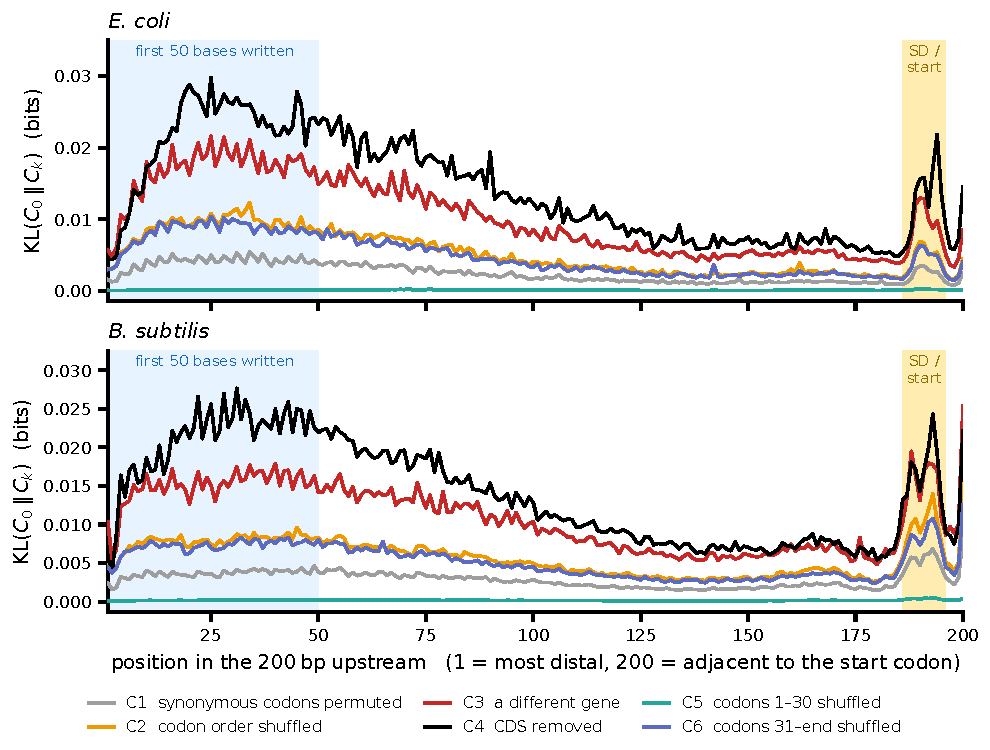
\includegraphics[width=\linewidth]{figures/supp_kl_perposition.pdf}
  \caption{\rev{\textbf{Where the CDS sensitivity sits along the upstream.}
  \emph{How this is assessed.} For one gene we give the model its real CDS and
  then walk along the real $200$\,bp upstream one base at a time, recording the
  four base probabilities the model predicts at each position. We repeat this with
  the CDS perturbed (C1--C6, Table~\ref{tab:conditions}) and the upstream
  unchanged, and plot the per-position KL divergence between the two sets of
  predictions (the summand of Eq.~\ref{eq:kl}, before the sum over positions).
  A larger value at a position means the model's expectation for that base
  depends on which gene follows. Position $1$ is the most distal base and the
  first one the model writes; position $200$ is adjacent to the start codon.
  \emph{What it shows.} The response is a decay from the prompt boundary, not a
  feature of the regulatory elements. The first $50$ positions hold $38$--$43\%$
  of the total in \emph{E.~coli} against a $25\%$ share of the window
  ($1.5$--$1.7\times$), whereas the Shine--Dalgarno and start-codon region
  (shaded, positions $186$--$196$) holds $0.84$--$0.94\times$ its share for every
  large perturbation. The exception is C5, which shuffles only codons $1$--$30$,
  the stretch adjacent to the Shine--Dalgarno: it is the smallest effect overall
  ($0.02$ bits) yet the only condition enriched at that region
  ($1.6\times$ in \emph{E.~coli}, $2.1\times$ in \emph{B.~subtilis}). Per-condition
  totals, peaks and enrichments are released in
  \texttt{results/supp\_kl\_perposition\_stats.csv}. Curves are averaged over
  genes; the spread across individual genes is not resolved here.}}
  \label{fig:klpos}
\end{figure}

\begin{table}[htbp]
  \centering
  \small
  \caption{\textbf{Promoter and Shine--Dalgarno placement by model.}
  Percentage of generations whose best PWM match lies within $\pm2$\,bp of the
  element's annotation, by sigma factor. Bold marks the best model per column;
  italic rows are natural sequence and shuffled model output. No model exceeds the
  scrambled control by more than a few points in any column, so the failure is not
  confined to $\sigma^{70}$.}
  \label{tab:upstream}
  \begin{tabular}{@{}lcccccc@{}}
    \toprule
    & \multicolumn{5}{c}{proximal box, by sigma factor} & Shine--Dalgarno \\
    \cmidrule(lr){2-6}\cmidrule(l){7-7}
    Model & $\sigma^{70}$ & $\sigma^{38}$ & $\sigma^{32}$ & $\sigma^{24}$ & $\sigma^{54}$ & all \\
    \midrule
    \emph{real sequence} & \emph{67.6} & \emph{63.4} & \emph{87.8} & \emph{68.8} & \emph{82.8} & \emph{78.6} \\
    \midrule
    Evo 1 (8k)   & 10.5 & 11.9 & 13.6 & 11.0 & 12.6 & \textbf{15.2} \\
    Evo 1 (131k) & 10.7 & 10.9 & \textbf{17.3} & \textbf{16.1} & 15.1 & 13.8 \\
    Evo 2      & \textbf{13.7} & 11.9 & 11.0 & 12.2 & \textbf{19.5} & 14.7 \\
    HyenaDNA   & 11.6 & 11.7 & 10.8 & 11.2 & 12.0 & 13.6 \\
    PromoGen2  & 10.8 & \textbf{12.5} & 15.3 & 11.2 & 13.3 & 12.4 \\
    \midrule
    \emph{scrambled control} & \emph{12.3} & \emph{12.2} & \emph{12.2} & \emph{12.8} & \emph{13.4} & \emph{14.5} \\
    \bottomrule
  \end{tabular}
\end{table}

\begin{figure}[htbp]
  \centering
  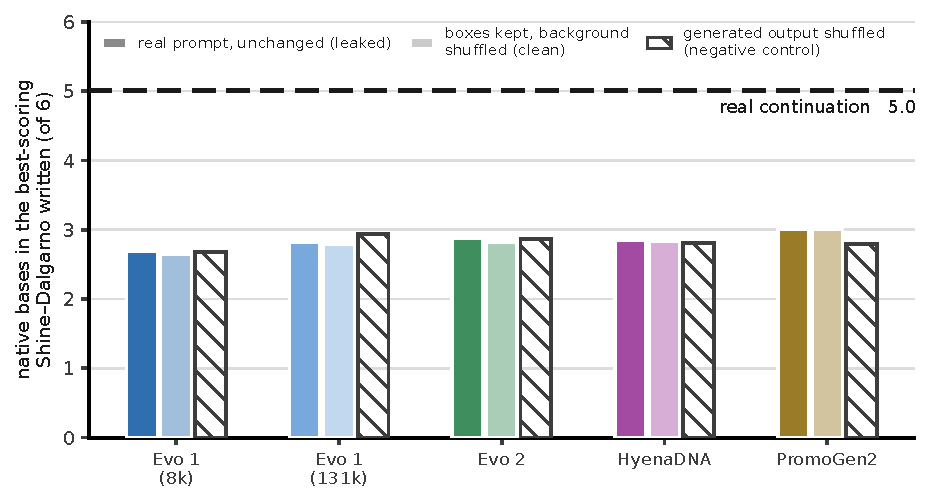
\includegraphics[width=0.82\linewidth]{figures/supp_sd_matches.pdf}
  \caption{\textbf{The best Shine--Dalgarno a model writes is not the right one.}
  Fig.~\ref{fig:upstream}C repeated for the Shine--Dalgarno task on all $681$
  genes: the highest-scoring SD PWM window in each generation, scored by how many
  of its six bases match that gene's annotated SD core. Bars are the leaked and
  clean prompt conditions and the shuffled-output negative control. The dashed
  line is the same scan on
  the real continuation ($5.01/6$). Every model scores $2.6$--$3.0$, and none
  exceeds its own shuffled output by more than $0.24$ bases.}
  \label{fig:sd-placement}
\end{figure}

\FloatBarrier

% =====================================================================
% =====================================================================
\section{Coding sequence as a positive control}
\label{app:cdscompletion}

The same models were asked to continue coding sequence instead of regulatory
sequence, under the same free-running decode. Figure~\ref{fig:cdscompletion}
shows the positionwise profiles, and Fig.~\ref{fig:positionblind} compares their
distance from real coding and upstream sequence.

\begin{figure}[htbp]
  \centering
  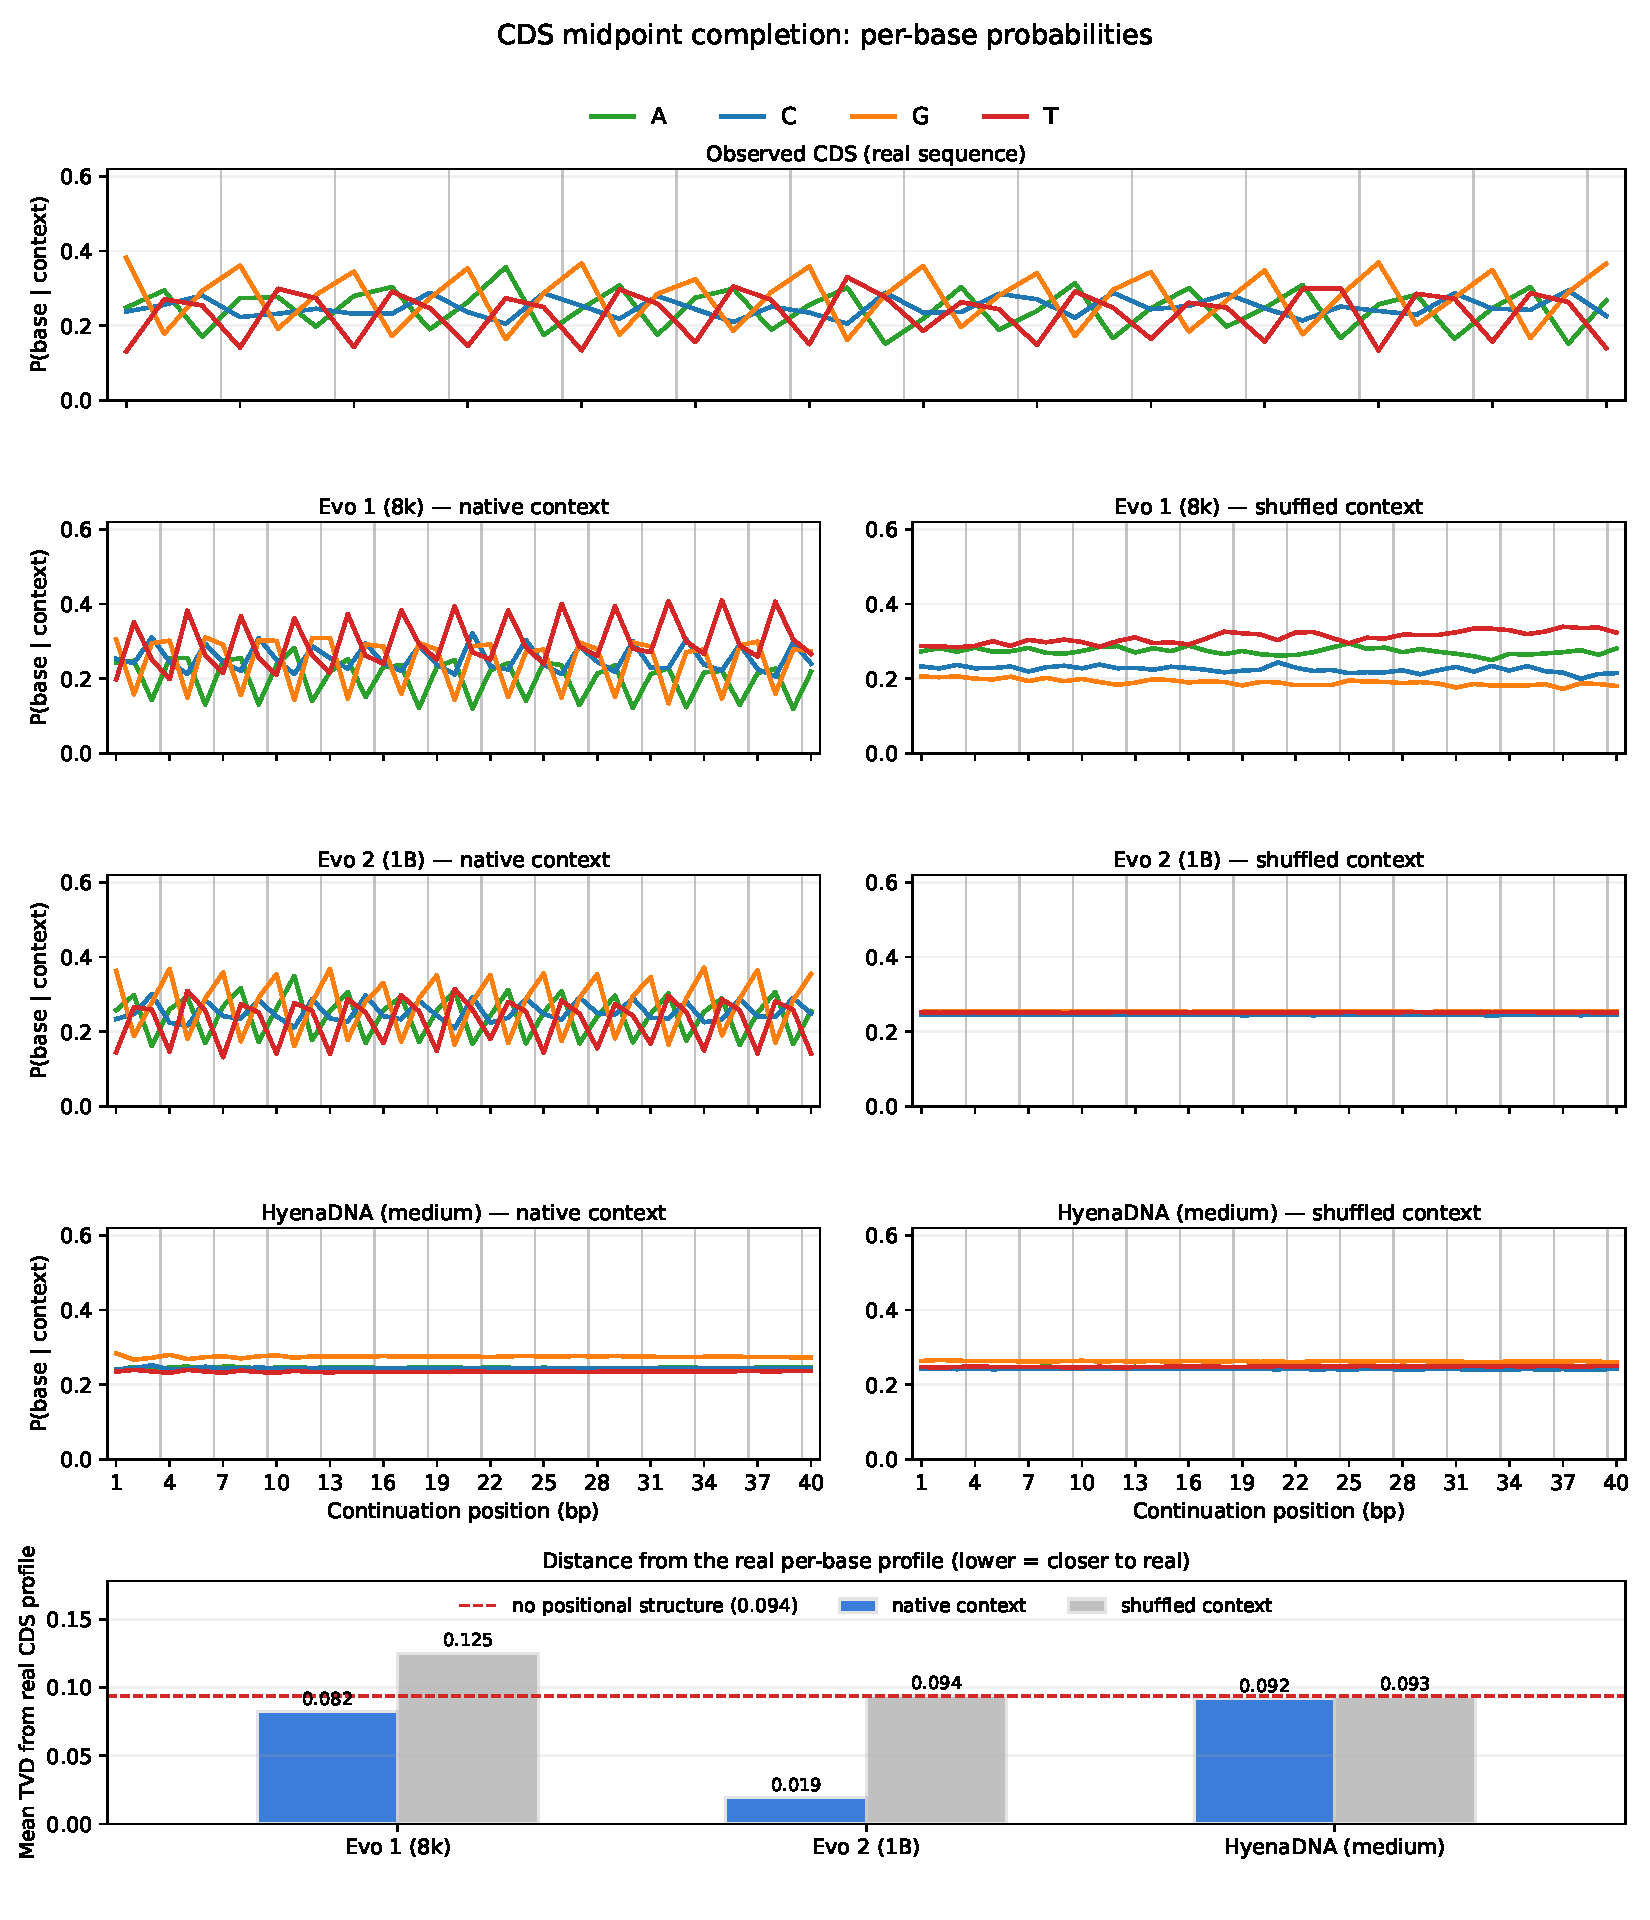
\includegraphics[width=\linewidth]{figures/supp_cds_completion_probabilities.pdf}
  \caption{\textbf{CDS midpoint completion: per-base probabilities.}
  Each of $672$ \emph{E.~coli} genes was cut at the midpoint of its coding
  sequence and continued for $40$\,bp ($1$ greedy plus $20$ sampled decodes per
  gene and condition). \textbf{Top:} probability of A, C, G and T at each
  continuation position in the real coding sequence. \textbf{Middle:} the same
  profiles for Evo\,1 (8k), Evo\,2 (1B) and HyenaDNA, prompted with the native
  context (left) or with a shuffled context (right). \textbf{Bottom:} mean total
  variation distance between each model's profile and the real one; $0$ means
  identical profiles. The dashed line ($0.094$) is the distance obtained by using
  the same overall base composition at every position.}
  \label{fig:cdscompletion}
\end{figure}

\begin{figure}[htbp]
  \centering
  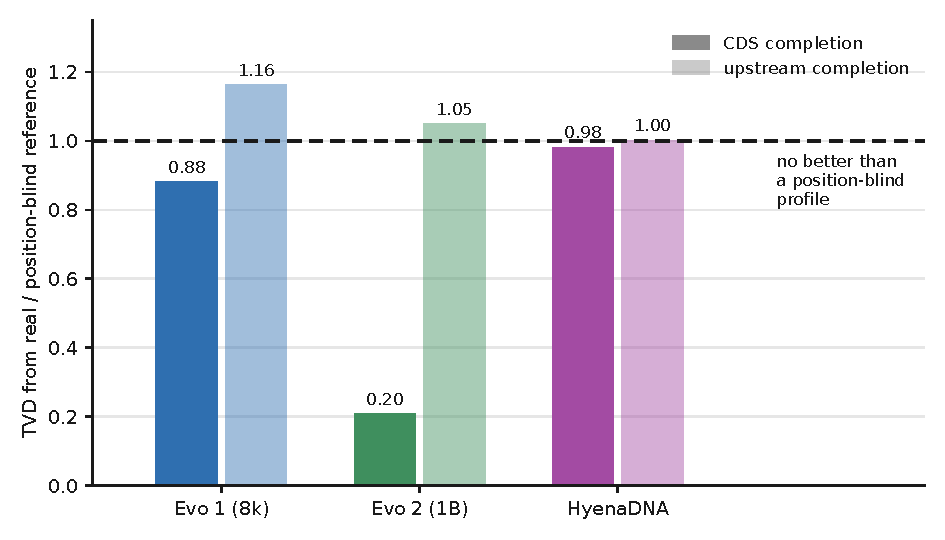
\includegraphics[width=0.82\linewidth]{figures/fig_cds_vs_upstream_gap.pdf}
  \caption{\textbf{The same models are further from real upstream sequence than
  from real coding sequence.} Mean total variation distance between each model's
  per-base profile and the real one,
  $\mathrm{TVD}(i)=\tfrac{1}{2}\sum_b|p_{\mathrm{model}}(i,b)-p_{\mathrm{real}}(i,b)|$,
  where $p(i,b)$ is the frequency of base $b$ at position $i$. TVD is $0$ when
  the generated and real profiles match. We divide it by the value obtained when
  the same overall base composition is used at every position
  ($0.094$ coding, $0.067$ upstream; dashed line). Below $1$ means positional
  structure was captured, $1$ composition alone, above $1$ that the composition is
  off as well; finite-sample noise alone gives $0.026$ and $0.031$. CDS completion: $672$
  \emph{E.~coli} genes cut at the CDS midpoint and continued for $40$\,bp.
  Upstream completion: $487$ $\sigma^{70}$ promoters over the $41$ positions
  following the distal box (the Fig.~\ref{fig:upstream}B window). PromoGen2 and
  Evo\,1 (131k) were not run on both windows and are omitted.}
  \label{fig:positionblind}
\end{figure}

\FloatBarrier

% The workshop requires appendices in the submission PDF rather than as a
% separate upload. This switch makes supplementary.tex omit its standalone
% preamble and bibliography while continuing the appendix lettering.
\newcommand{\ICBINBSupplementInMain}{}
% !TeX root = main.tex
% =====================================================================
% Supporting appendices for
%   "Composition Without Grammar: Next-Token Models Miss Regulatory
%    Structure in Bacterial DNA"  --  ICBINB-BIO @ NeurIPS 2026
% ---------------------------------------------------------------------
% SUBMISSION: this file is \input by main.tex after Appendix B, so its sections
% continue the appendix lettering in the same PDF. Compiling supplementary.tex
% alone is only for local inspection; do not submit a separate appendix PDF.
% =====================================================================
\ifdefined\ICBINBSupplementInMain
  \clearpage
  \FloatBarrier
\else
\documentclass{article}

\PassOptionsToPackage{numbers,sort&compress}{natbib}
\usepackage[dblblindworkshop]{neurips_2026}
\workshoptitle{I Can't Believe It's Not Better (ICBINB): Failure Modes of AI in Biology}

\usepackage[utf8]{inputenc}
\usepackage[T1]{fontenc}
\usepackage{hyperref}
\hypersetup{hidelinks}
\usepackage{url}
\usepackage{booktabs}
\usepackage{amsmath,amssymb,amsfonts}
\usepackage{nicefrac}
\usepackage{microtype}
\usepackage{xcolor}
\usepackage{graphicx}
\usepackage{placeins}

% Float placement: identical to main.tex, so the standalone build lays the
% figures out the way they appear in the submission PDF.
\renewcommand{\topfraction}{0.95}
\renewcommand{\bottomfraction}{0.7}
\renewcommand{\textfraction}{0.05}
\renewcommand{\floatpagefraction}{0.90}
\setcounter{topnumber}{2}
\setcounter{totalnumber}{4}

\renewcommand{\thesection}{\Alph{section}}
\numberwithin{figure}{section}
\numberwithin{table}{section}
\numberwithin{equation}{section}

\title{Supporting Appendix\\[0.4em]
\large Composition Without Grammar: Next-Token Models Miss Regulatory
Structure in Bacterial DNA}

\author{Marc Augustine Sojerido Amil \and Aleksej Zelezniak}

\begin{document}
\maketitle

This document collects supporting analyses for the main paper. In the submitted
PDF these sections continue after Appendix B rather than appearing as a separate
file.
\fi

% Camera-ready revision marking. Defined here with \providecommand so that this
% file also compiles standalone; main.tex defines the same macro.
\providecommand{\rev}[1]{\begingroup\color{red}#1\endgroup}

% =====================================================================
\section{The gene--upstream association of Fig.~1A}
\label{app:fig1a}

\paragraph{Pairs and controls.} We paired $727$ \emph{E.~coli} K-12 singletons
with singleton orthologues from MMseqs2 Gammaproteobacterial families, requiring
$\ge30\%$ BLASTP identity, $\ge70\%$ coverage and a full $200$\,bp upstream. This
gave $22{,}393$ pairs from $408$ genomes. Controls were unrelated singletons from
the same target genome, length-matched to $\pm10\%$, thereby matching genome
composition and phylogenetic distance while removing homology.

\rev{\paragraph{Why conserved gene order does not drive this panel.} Both filters
above are applied to every gene on both sides of every pair, and together they
rule out the obvious synteny confound. ``Singleton'' means an operon size of one,
so the gene is not co-transcribed with a neighbour; ``a full $200$\,bp upstream''
means the annotated distance to the nearest upstream feature is at least
$200$\,bp, so the window stops before the neighbouring gene and contains no
neighbouring coding sequence. A window here is therefore intergenic by
construction, and conserved gene order cannot produce upstream similarity by
placing a conserved CDS inside it. The controls inherit the same two filters, so
test and control pairs are matched on gene architecture as well as on genome
composition, phylogenetic distance and upstream length. The coverage figures
quoted in Appendix~\ref{app:cds-composition} ($41\%$ and $32\%$ of windows clear
of the nearest upstream feature) describe the CDS-prompted benchmark, which
applies no such distance requirement, and do not apply to this panel.

One weaker version of the concern does survive. Clearing the neighbouring
\emph{gene} does not clear shared regulatory architecture: where a gene and its
orthologue both lie downstream of a divergently transcribed neighbour, the
conserved sequence in the window may be that neighbour's promoter rather than the
focal gene's. This remains regulatory sequence, but it is not necessarily
evidence of coevolution with the focal CDS.}

\paragraph{Upstream similarity ($D_2^*$).} A direct $4$-mer comparison can be
misleading because two AT-rich sequences share many short words even when they
are unrelated. We therefore compare observed counts with those expected from
each sequence's own background composition. For a $4$-mer $w$, $X_w$ is its
observed count and $\mathbb{E}[X_w]$ its expected count. The expectation uses an
order-$2$ Markov model, which predicts each base from the previous two bases:
$\mathbb{E}[X_w]=N(w_{1:3})N(w_{2:4})/N(w_{2:3})$, where $N(u)$ counts substring
$u$ and the subscripts select the first three, last three and middle two bases of
$w$. We then calculate
%
\begin{equation}
\tilde{X}_w = \frac{X_w - \mathbb{E}[X_w]}{\sqrt{\mathbb{E}[X_w]}},
\qquad
D_2^{*} = \frac{\sum_w \tilde{X}_w \tilde{Y}_w}
               {\sqrt{\sum_w \tilde{X}_w^{2}}\;\sqrt{\sum_w \tilde{Y}_w^{2}}},
\end{equation}
%
Here, $\tilde X_w$ is positive when $w$ occurs more often than expected and
negative when it occurs less often; $\tilde Y_w$ is the same value for the second
sequence. $D_2^*$ compares these corrected patterns across all $256$ $4$-mers:
$1$ means the patterns match and $0$ means no agreement. It therefore measures
similarity beyond that explained by background base composition.

\paragraph{Third-position identity.} A codon contains three bases, and changes at
its third base often do not change the encoded amino acid. For each aligned gene
pair, we therefore calculate the fraction of codons with the same third base,
using pairs with at least $30$ aligned codons. A high value indicates more closely
related coding sequences and a low value greater evolutionary divergence. This is
the $x$ axis in Fig.~1A and measures relatedness, not gene function.

% =====================================================================
\section{The upstream-only benchmark}
\label{app:benchmark-composition}

Not all five sigma factors build promoters from $-35$/$-10$ elements
($\sigma^{54}$ uses $-24$/$-12$), so we write \emph{distal} and \emph{proximal}
box throughout. Figure~\ref{fig:benchmark-composition} summarizes the dataset and
controls, Fig.~\ref{fig:sigma-logos} shows the box motifs, and
Fig.~\ref{fig:spacerhist} shows the spacer-length distributions.

\begin{figure}[htbp]
  \centering
  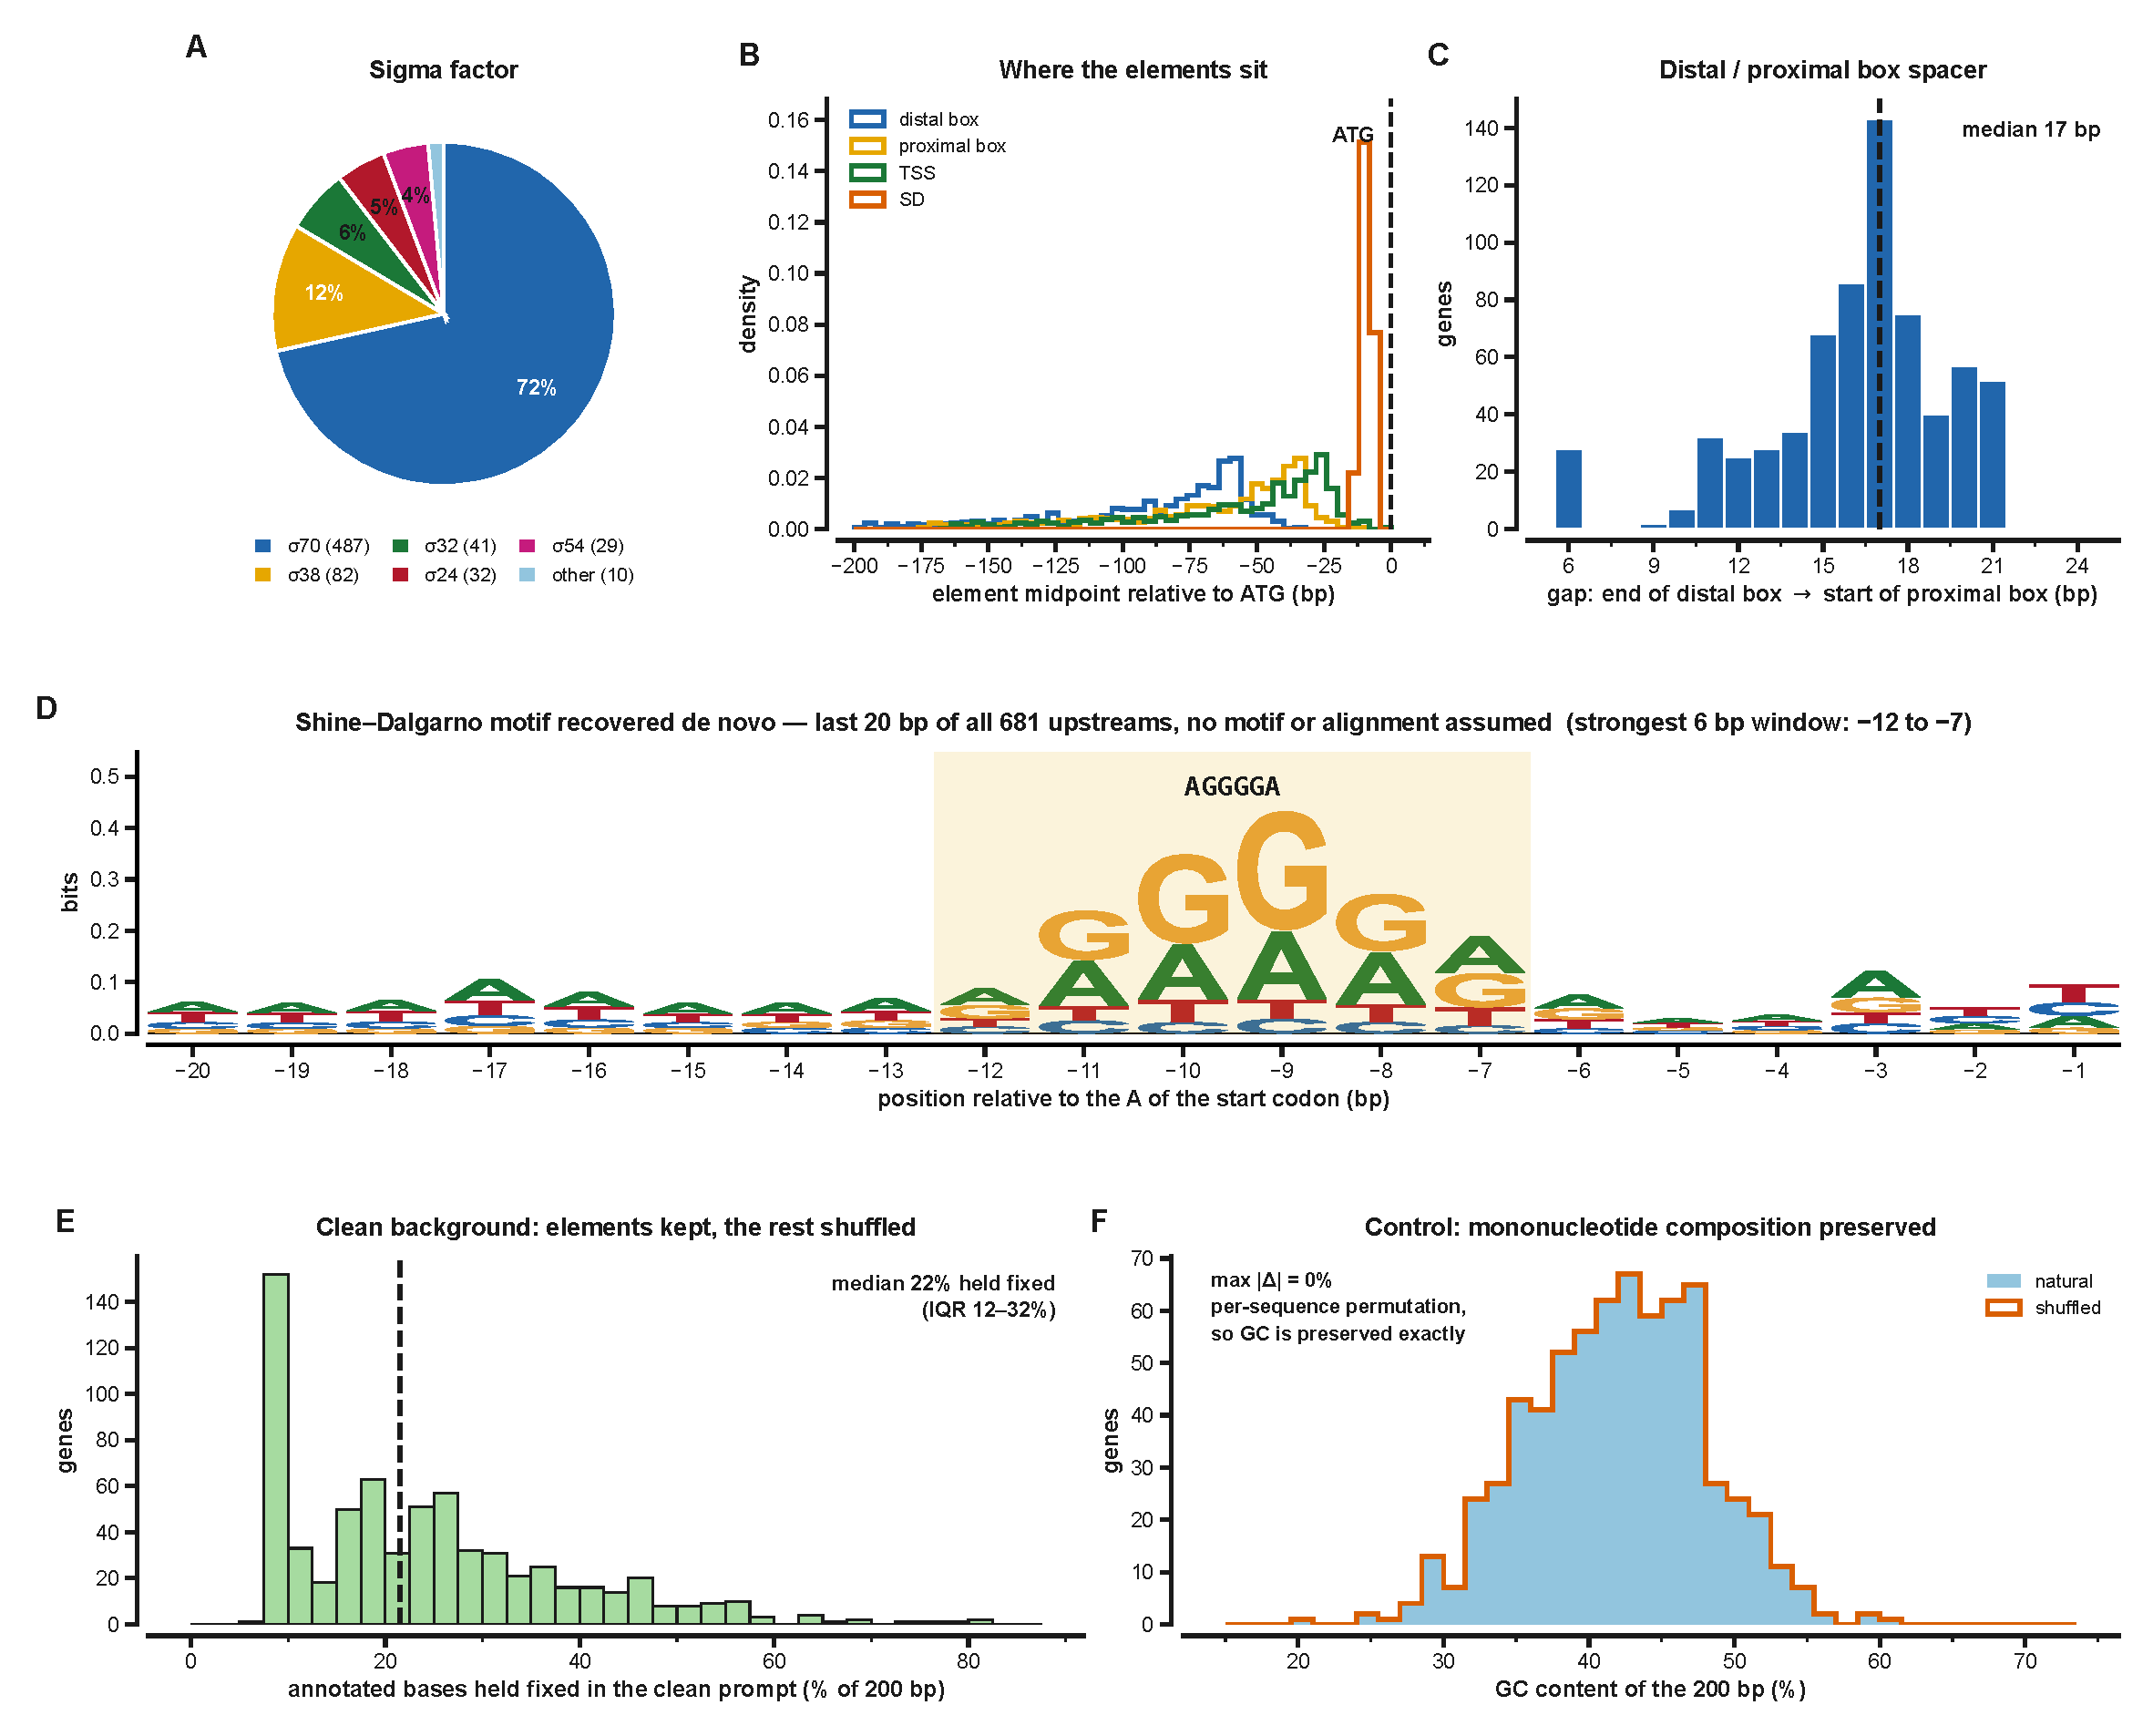
\includegraphics[width=0.95\linewidth]{figures/upstream_only_dataset_supp.pdf}
  \caption{\textbf{Composition and controls of the upstream-only benchmark.}
  $681$ RegulonDB-annotated \emph{E.~coli} genes with up to $200$\,bp before the
  start codon. \textbf{(A)} Sigma-factor counts; promoter-box analyses use the 671
  genes in the five displayed factors, while one $\sigma^{28}$ and nine unassigned
  genes remain in Shine--Dalgarno analyses. \textbf{(B)} Annotated element
  midpoints relative to the start codon. \textbf{(C)} Distal-to-proximal box
  spacing. \textbf{(D)} Information logo for the final $20$\,bp.
  \textbf{(E)} Fraction of each clean prompt held fixed as an annotated element.
  \textbf{(F)} Natural and clean-prompt GC content. The Shine--Dalgarno emerges de
  novo in (D) with no motif assumed, and the clean background holds every annotated
  element at its real position (E) while preserving mononucleotide composition
  exactly (F), so a score against it cannot be explained by composition.}
  \label{fig:benchmark-composition}
\end{figure}

\begin{figure}[htbp]
  \centering
  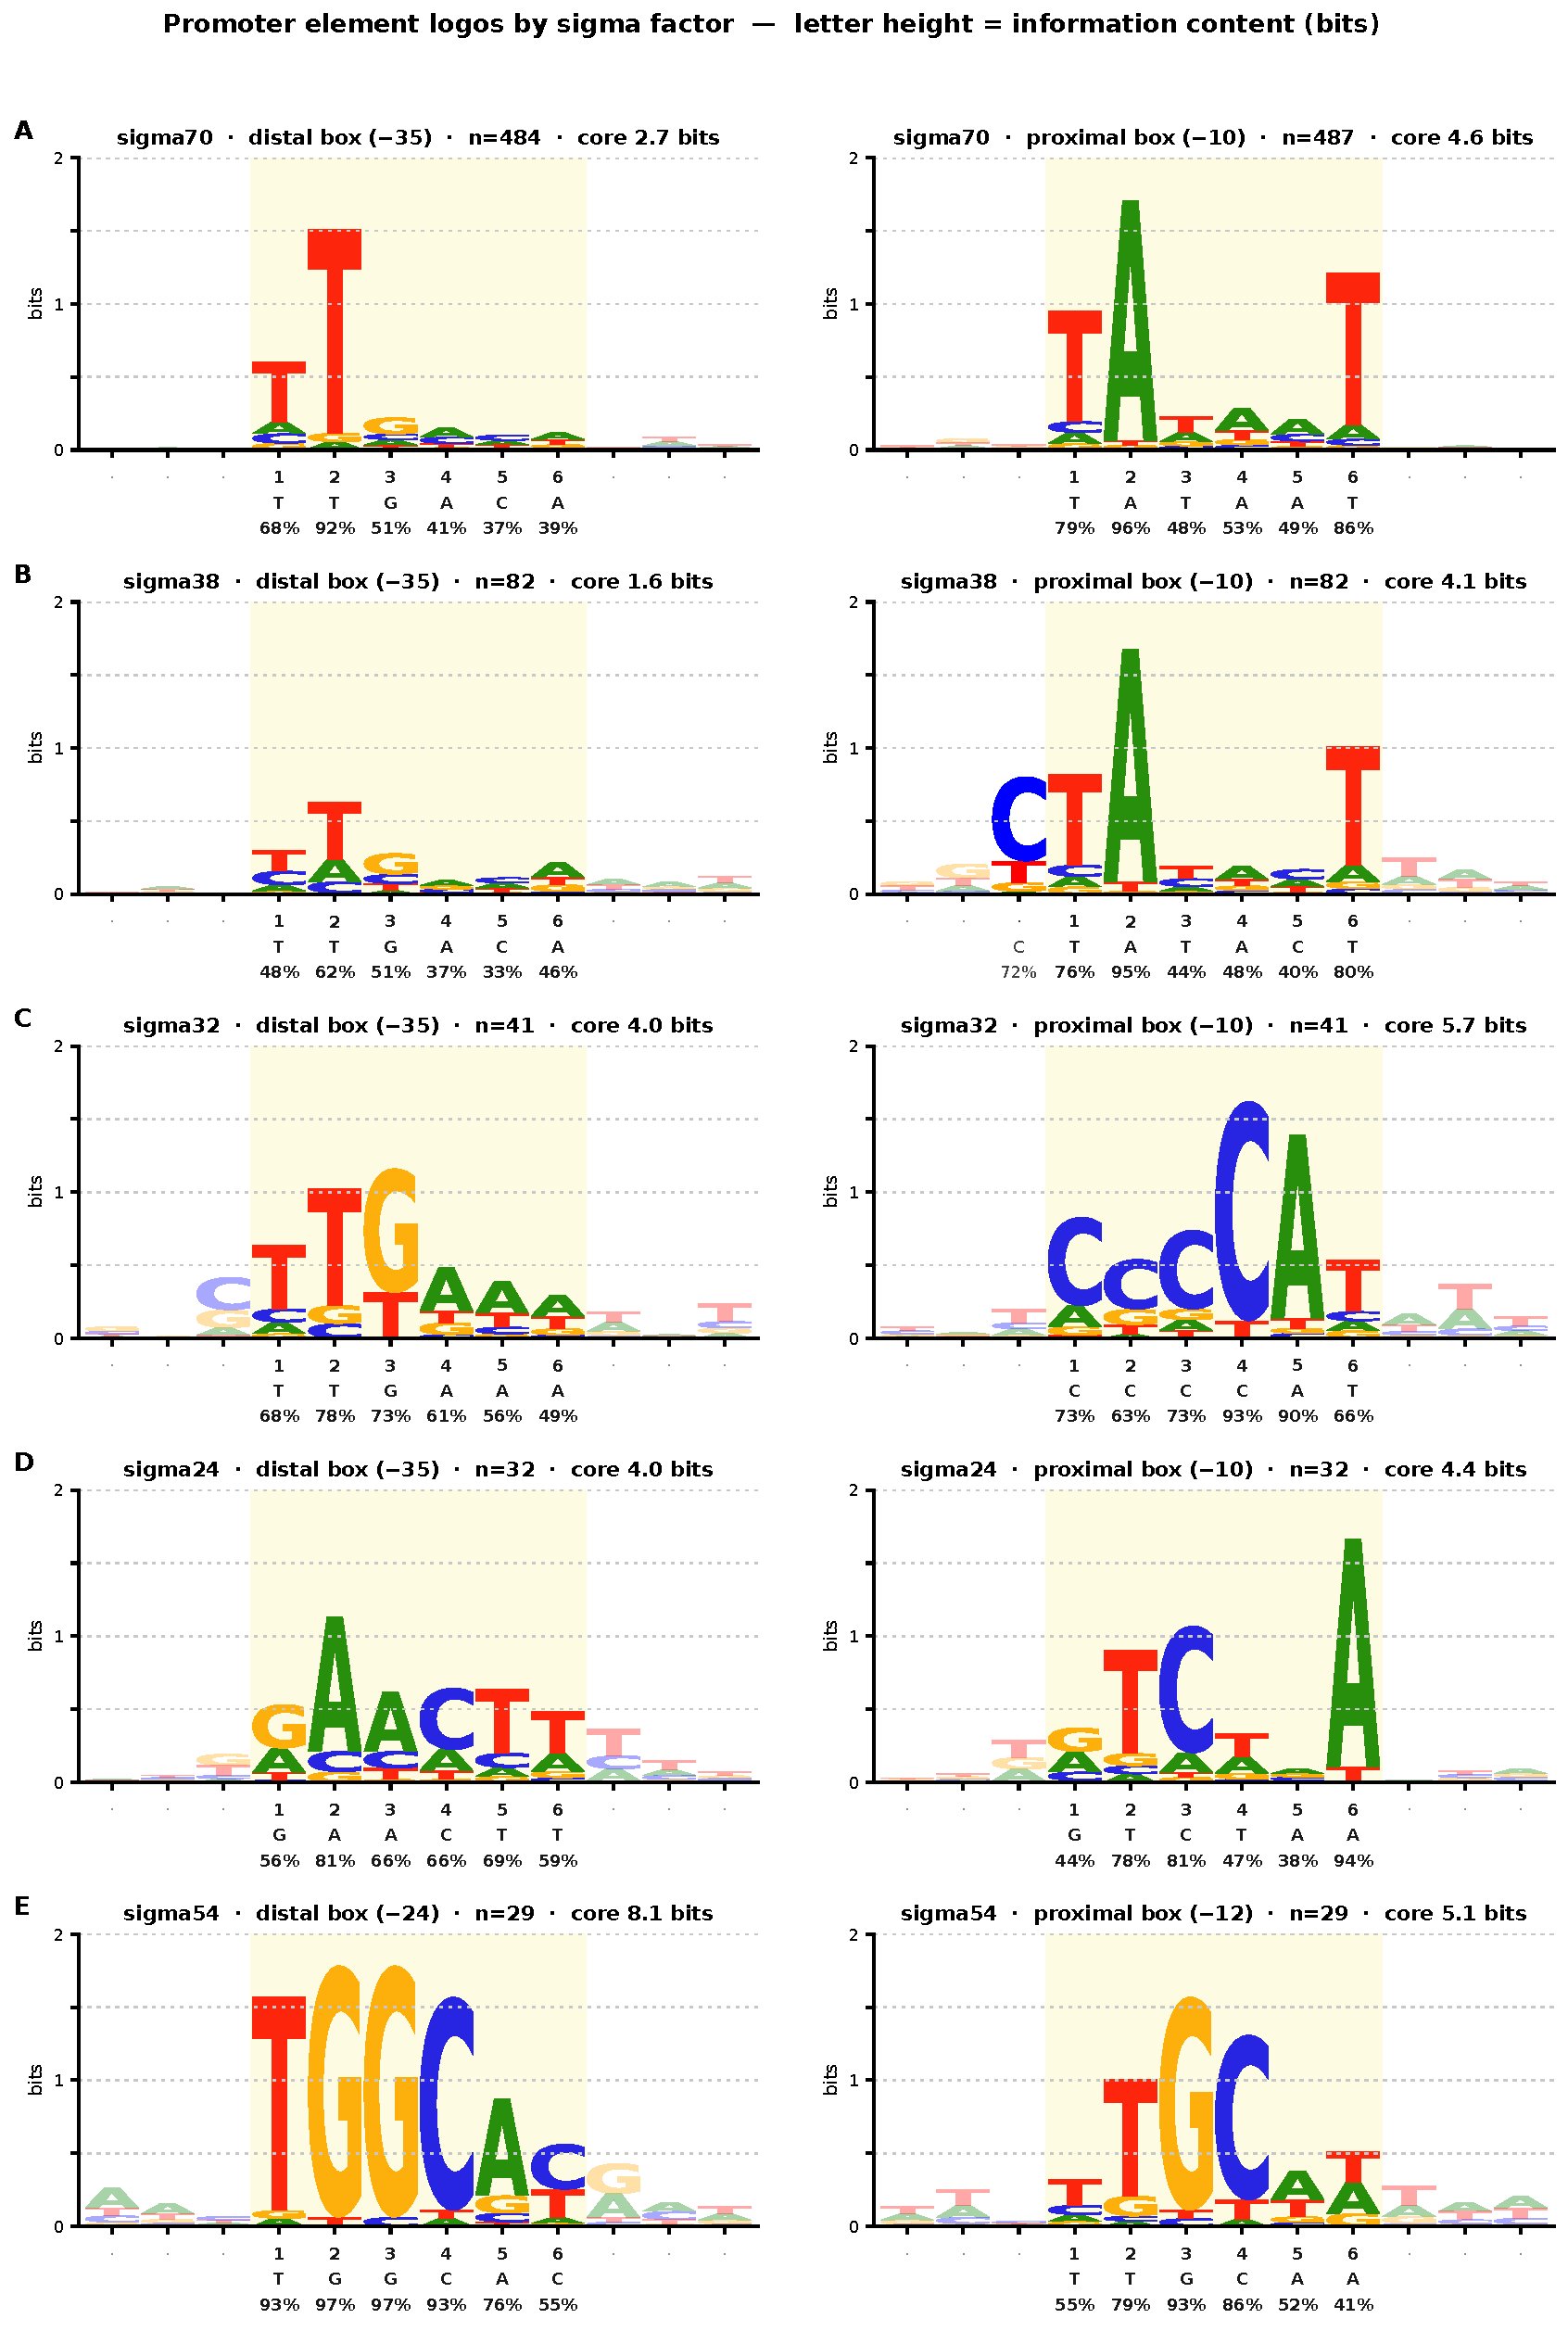
\includegraphics[width=0.88\linewidth]{figures/upstream_only_logos.pdf}
  \caption{\textbf{Promoter-box logos by sigma factor.}
  Information logos for distal and proximal boxes in RegulonDB-annotated
  \emph{E.~coli} upstreams ($n\ge 25$ per factor). Six-base cores are shaded and
  three-base flanks are faded; the modal base and frequency are printed below each
  core position. Windows are anchored at the distal box's $5'$ end and the
  proximal box's $3'$ end; the benchmark reproduces the published consensus for
  every factor.}
  \label{fig:sigma-logos}
\end{figure}

% =====================================================================
\begin{figure}[htbp]
  \centering
  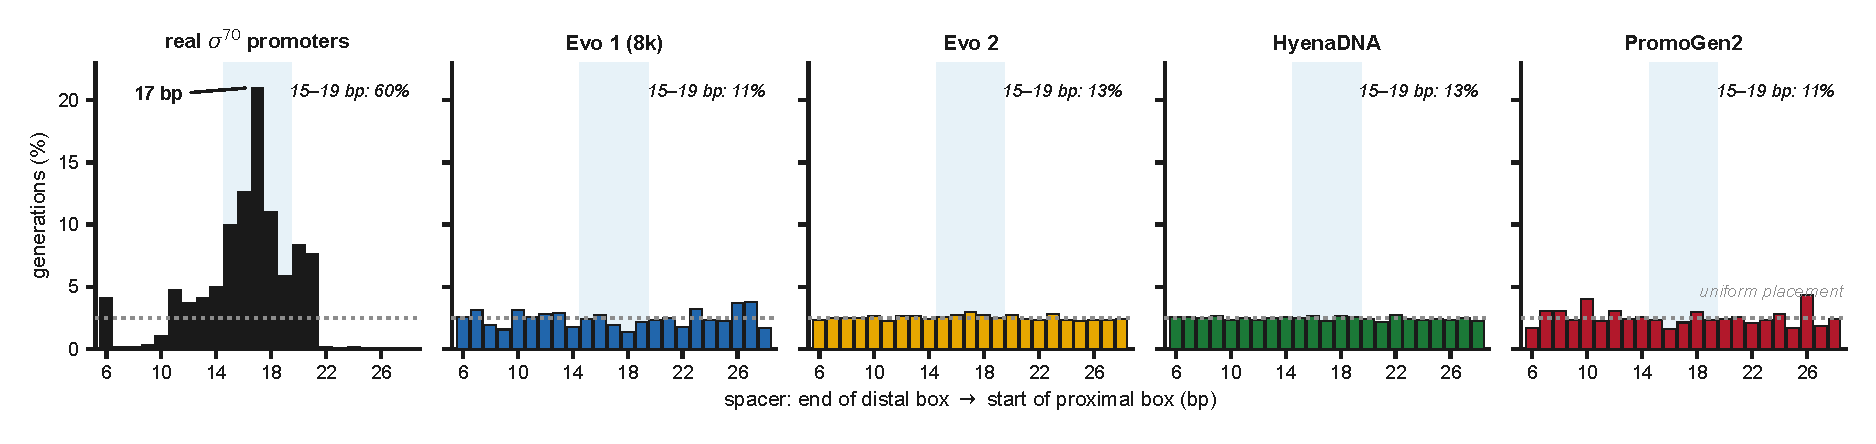
\includegraphics[width=\linewidth]{figures/supp_spacer_histograms.pdf}
  \caption{\textbf{The spacer distribution, one histogram per model.} Each model's
  best-scoring proximal-box position, read as a spacer from the distal box, on a
  shared $y$-axis. Real $\sigma^{70}$ promoters concentrate at $17$\,bp; every model
  spreads the spacer almost uniformly. Shading marks the canonical $15$--$19$\,bp
  window, the dotted line uniform placement ($2.5\%$ per offset), and the inset
  number the fraction inside the canonical window. Real promoters fall in the
  canonical window $60.5\%$ of the time and at exactly $17$\,bp $21.0\%$ of the
  time; the models give $10.7$--$13.5\%$ and $2.0$--$3.0\%$, against $12.5\%$ and
  $2.5\%$ for uniform placement. Presence is not the failing quantity: the scan
  finds a box in $93$--$97\%$ of generations and in $95$--$97\%$ of shuffles of
  those same generations, because an AT-rich stretch supplies a proximal-box-like
  hexamer by chance.}
  \label{fig:spacerhist}
\end{figure}


% =====================================================================
\FloatBarrier
\section{What the models were trained on}
\label{app:traincomp}

Non-coding bases---those outside predicted coding regions---are an upper bound on
what a model could have learned promoters from.

\begin{figure}[!htbp]
  \centering
  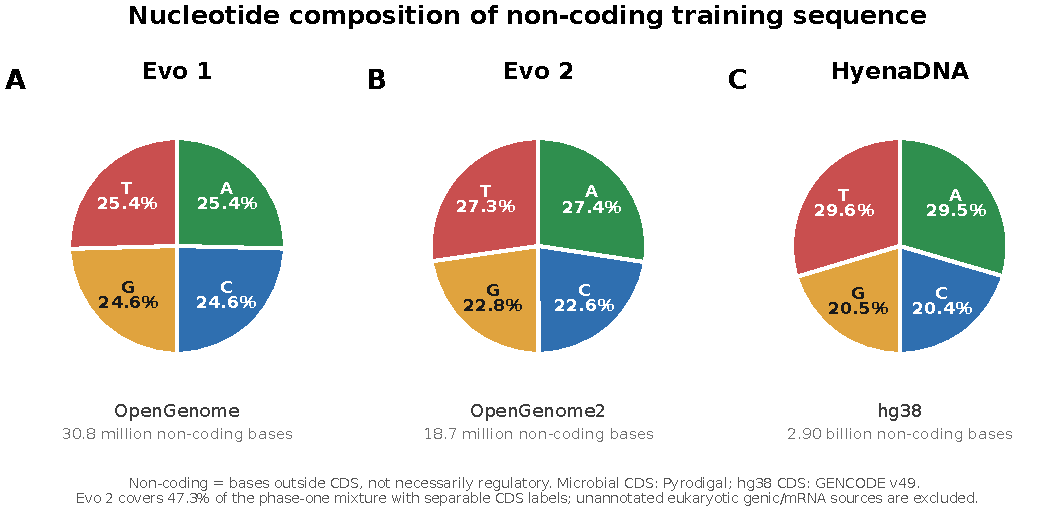
\includegraphics[width=\linewidth]{figures/supp_training_composition.pdf}
  \caption{\textbf{Nucleotide composition of the non-coding sequence in each
  model's training corpus.} Bases outside predicted CDS intervals, sampled
  reproducibly from each released corpus. \textbf{(A)}~Evo\,1 (OpenGenome).
  \textbf{(B)}~Evo\,2 (OpenGenome2), restricted to the $47.3\%$ of the phase-one
  mixture whose records carry separable CDS labels; unannotated eukaryotic
  genic and mRNA sources are excluded. \textbf{(C)}~HyenaDNA (hg38). PromoGen2 is
  omitted: it is trained on curated promoter sequence, not whole genomes. The
  corpora differ ($50.8\%$, $54.7\%$ and $59.2\%$ AT) but the outputs do not
  ($60.4\%$, $57.7\%$ and $59.7\%$, against $61.5\%$ in real \emph{E.~coli}
  upstreams), so matching the composition of a bacterial upstream is a low bar.}
  \label{fig:traincomp}
\end{figure}

% =====================================================================
\FloatBarrier
\section{Composition of the CDS-prompted benchmark}
\label{app:cds-composition}

The benchmark contains protein-coding, in-frame singletons of at least $30$
codons with a complete $200$\,bp upstream: $1{,}885$ from \emph{E.~coli} and
$1{,}272$ from \emph{B.~subtilis}. Only $41\%$ and $32\%$ of these windows are
clear of the nearest upstream feature, so overlap is a stratifier; restricting
the analysis to singletons limits inference to independently regulated genes.
\rev{This coverage figure applies to the CDS-prompted benchmark only. The Fig.~1A
pairs additionally require at least $200$\,bp to the nearest upstream feature
(Appendix~\ref{app:fig1a}), so every window in that panel is clear.}

The seven conditions are defined in Table~\ref{tab:conditions}. C1 and C2
rearrange codons, C3 substitutes another gene and C4 removes the CDS. C5 shuffles
the first $30$ codons and C6 the remainder, contrasting the region nearest the
ribosome-binding site with the region nearest the generation point. Cross-gene
upstream identity is near the composition floor ($0.255$ and $0.269$), so a
species-generic upstream is not a gene-specific match.

\begin{table}[htbp]
  \centering
  \footnotesize
  \caption{\textbf{The seven CDS perturbation conditions.} Percentages are mean
  nucleotide changes in \emph{E.~coli}/\emph{B.~subtilis}. The start codon is
  fixed; shuffled conditions preserve length, codon counts and GC, while C3 is
  length-matched and GC-matched in the mean. KL results are in
  Table~\ref{tab:kl}; C2 is shown in Fig.~\ref{fig:cds}C.}
  \label{tab:conditions}
  \begin{tabular}{@{}llcc@{}}
    \toprule
    & CDS given to the model & nt changed (E/B) & CDS GC vs.\ C0 \\
    \midrule
    C0 & the real CDS (reference)                      & ---            & --- \\
    C1 & synonymous codons permuted, protein unchanged & $20.0/20.6\%$  & identical \\
    C2 & codon order shuffled                          & $72.0/71.2\%$  & identical \\
    C3 & a different, length-matched gene's CDS        & $71.9/71.9\%$  & matched in the mean \\
    C4 & removed entirely                              & ---            & --- \\
    C5 & codons 1--30 shuffled; remainder fixed        & $10.7/11.9\%$  & identical \\
    C6 & codons 31--end shuffled; first 30 fixed       & $60.8/58.7\%$  & identical \\
    \bottomrule
  \end{tabular}
\end{table}

\ifdefined\ICBINBSupplementInMain
  \FloatBarrier
\else
  \bibliographystyle{plainnat}
  \bibliography{Literature_Sources/references}
  \end{document}
\fi


\end{document}
